%!TEX TS-program = xelatex

\documentclass[9pt,paper=a6,twoside=true,BCOR=10mm,DIV=calc]{scrbook}
\usepackage{incgraph,microtype,tikz,colortbl,pdflscape,moresize,lmodern,enumitem,wrapfig}

\usepackage{relsize}

% How to use custom fonts:
% https://www.overleaf.com/learn/latex/Questions/I_have_a_custom_font_I%27d_like_to_load_to_my_document._How_can_I_do_this%3F
% Basically this boils down to:
% 1. XeLaTeX
% 2. \usepackage{fontspec}
% 3. \setmainfont{}
%    \setsansfont{}
%    \setmonofont{}
% \usepackage{fontspec}
% \setmainfont[BoldFont={GT-America-Mono-Bold.OTF}]{GT-America-Mono-Regular.OTF}
% \setsansfont{GT-America-Mono-Regular.OTF}
% \setmonofont{GT-America-Mono-Regular.OTF}

% The following three lines will not be required any more.
% \usepackage[utf8]{inputenc}
% \usepackage[tt=false]{libertine}
% \usepackage{tgbonum}
% \renewcommand{\ttdefault}{cmtt}

\areaset[10mm]{85mm}{128mm}
\setlength{\footskip}{6mm}

\usepackage{array}
\newcolumntype{L}[1]{>{\raggedright\let\newline\\\arraybackslash\hspace{0pt}}m{#1}}
\newcolumntype{C}[1]{>{\centering\let\newline\\\arraybackslash\hspace{0pt}}m{#1}}
\newcolumntype{R}[1]{>{\raggedleft\let\newline\\\arraybackslash\hspace{0pt}}m{#1}}

\usepackage{ifoddpage}
\newcommand{\startonleftevenpage}{
\clearpage
\checkoddpage
\ifoddpage
\else
\newpage
\fi
}
\newcommand{\startonrightoddpage}{
\clearpage
\checkoddpage
\ifoddpage
\newpage
\else
\fi
}

\hypersetup{
    colorlinks,
    linkcolor=, %linkcolor={red!50!black},
    citecolor={blue!50!black},
    urlcolor={blue!80!black}
}

\title{SIGMOD 2019}

\begin{document}

% normal \emph{italic}, \textbf{bold} and \textbf{\emph{bold italic}}

\incgraph[paper=document,options={width=105mm}]{images/cover.pdf}
\setlength\parindent{0pt}

%!TEX root = booklet.tex

\section{Welcome to ACM SIGMOD/PODS 2019!}

This year, SIGMOD/PODS is held in the city center of Amsterdam, capital of The Netherlands. Amsterdam is an internationally oriented city, home to people with origins from all over the world. This used to be already the case even back in the 16th and 17th century, when Amsterdam was the world's biggest trading and financial center; establishing the world's first stock exchange in 1602.

SIGMOD/PODS 2019 is held in the original Amsterdam Stock and Commodities Exchange, constructed by Dutch architect Berlage between 1896 and 1903, which now serves as the well-equipped Amsterdam Conference Center. This architect and his apprentices (the school of Berlage) left an important mark on the city, being responsible for a major expansion of the city in the early 20th century. The sculptures and drawings in the Exchange building refer to the people behind the commodities traded in the various rooms (``Effecten'' - stock; ``Graan'' - grains), e.g., depicting farmers in the grain exchange room; as a reminder that trading affects society.

Amsterdam is a city that offers many cultural activities, including the world-famous classical Concertgebouw Orchestra, as well as many museums (Amsterdam Museum, Rijksmuseum, Rembrandthuis, Anne Frank Huis). In a slight break with SIGMOD tradition, the SIGMOD opening reception will be held one day later, on Tuesday night, when the SIGMOD/PODS attendees will have exclusive access to the Van Gogh museum. The Wednesday conference dinner is organized across the water in Amsterdam North, in Noorderlicht Cafe in a festival-like environment. This used to be harbour area and was less-populated and industrial, but in the recent decade has become a hotspot for nightlife activities. Amsterdam is also increasingly a hub for data science companies and services, with multiple universities and CWI in the vicinity; which all participate in the organization of SIGMOD/PODS 2019. On Thursday night, after the SIGMOD program finishes, there will be a meetup of Amsterdam Data Science, where the local data science community will be able to mingle with our data management research community.

\vspace{-2mm}
\subsubsection*{Overview of SIGMOD 2019}
\vspace{-1mm}
The SIGMOD 2019 Research Program Committee consists of the Program Chair, two Program Vice Chairs, a core committee with 37 members, and a regular committee with 98 members. During the reviewing period, we solicited additional reviews from 16 external reviewers and occasional input from 10 assistant reviewers. The committee received 430 submissions, out of which 12 were desk-rejected (i.e., without review). There was no bidding; instead, reviewer assignments were made using input from Microsoft's Conference Management System, the Toronto Paper Matching System, and the reviewers' background (the detailed assignment procedure is described in a paper which has been submitted for publication to SIGMOD Record). The core committee members had (roughly) double the reviewing load of the regular committee members, and in addition acted as discussion leaders and meta-reviewers for their assigned papers. There were two rounds of submissions, with deadlines in July and November, respectively. Initially, each paper received three reviews. At this point authors could read the reviews and provide feedback about potential factual errors (disclosed to the reviewers) or sensitive issues about potential mishandling (confidentially to the chair). Two additional reviews were solicited for a paper if (a) the reviewers' expertise level was suboptimal, or (b) if there was significant score discrepancy in the first three reviews, or (c) if it was heading for rejection but had received a weak accept (or higher) by at least one reviewer. Papers were discussed extensively online; 10 were accepted based on the first round of reviews, while 311 were rejected. The authors of the remaining 97 papers were asked to revise their papers to address reviewers' criticisms; 78 revisions were ultimately accepted for a total of 88 papers which are presented in the research track. Finally, 12 papers were shepherded after acceptance to guarantee that the camera-ready version addresses all of the reviewers' comments.

\vspace{-2mm}
\subsubsection*{Overview of PODS 2019}
\vspace{-2mm}
The PODS Program committee consists of 24 members, including the chair. PODS submissions received at least 4 reviews; papers that include PC members among their authors received at least 5 reviews, and higher standards apply for their acceptance.  As in previous years, Easychair was used as the conference management tool for PODS. Also, as in previous years, PODS operated with two submission cycles. The first cycle allowed for the possibility of papers being revised and resubmitted. For the first cycle, 36 papers were submitted, 4 of which were directly selected for inclusion in the proceedings, and 8 were invited for a resubmission after a revision. The quality of most of the revised papers increased substantially with respect to the first submission, and all of the revised papers were selected for the proceedings. For the second cycle, 51 papers were submitted, 17 of which were selected, resulting in 29 papers selected overall from a total number of 87 submissions. The Best Paper and Best Student Paper awards, as well as the Gems of PODS talks and invited tutorials, were selected by a subcommittee of the PC, while the Alberto-Mendelzon Test-of-Time award winners were chosen by a separate committee appointed by the PODS Executive Committee.

~\\~

{\small%
\setlength{\tabcolsep}{0pt}
\begin{tabular*}{\textwidth}{@{\extracolsep{\fill}}ll}
\textbf{Stefan Manegold, Peter Boncz} & \textbf{Dan Suciu}           \\
\emph{SIGMOD'19 General Chairs}       & \emph{PODS'19 General Chair} \\
CWI, Netherlands                      & University of Washington     \\
 ~ & ~ \\
\textbf{Anastasia Ailamaki}           & \textbf{Christoph Koch}      \\
\emph{SIGMOD'19 Program Chair}        & \emph{PODS'19 Program Chair} \\
EPFL, Switzerland                     & EPFL, Switzerland            \\
\end{tabular*}
}

% %!TEX root = booklet.tex

\clearpage
\section*{WLAN}

Preferably, just use the {\em EDUROAM} network if you have eduroam access. Otherwise, follow the instructions below:

\vspace{5mm}
\begin{center}
%\fbox {
    
\includegraphics[width=30mm, trim=12mm 10mm 12mm 10mm, clip]{images/mwn-events.pdf}
%}
\end{center}

\vspace{5mm}
\begin{sloppypar}
\textbf{Wi-Fi-Guide for mwn-events} \\
Wi-Fi name (SSID): \texttt{mwn-events} \\
Username: \texttt{VLDB2017} \\
Password: \texttt{YTnO6kdF} \\
Valid from \texttt{Fri Aug 25 06:00 2017} to \texttt{Sat Sep 9 23:59 2017}

\vspace{2mm}
Configuration profiles for wireless network access are available via
the QR code or this URL:\\
\url{https://www.lrz.de/wlan} (follow the link mwn-events)
Access to this site is available via the open Wi-Fi (the SSID) "lrz".
\end{sloppypar}

\newpage
\section*{Our Sponsors}

\subsection*{Diamond Sponsor}

\newcommand{\sponsoricon}[1]{{\includegraphics[width=2cm,height=10mm,keepaspectratio]{#1}}}

\renewcommand{\arraystretch}{1.3}

\begin{tabular}{C{\linewidth}}
% \sponsoricon{sponsoricons/facebook}

\includegraphics[width=3cm,height=2cm,keepaspectratio]{sponsoricons/facebook}
\end{tabular}

\subsection*{Platinum Sponsors}

\begin{tabular}{C{.3\textwidth}C{.3\textwidth}C{.3\textwidth}}
\sponsoricon{sponsoricons/elsevier}
&
\sponsoricon{sponsoricons/microsoft}
&
\sponsoricon{sponsoricons/morgan-claypool}
\\
\sponsoricon{sponsoricons/oracle}
&
\sponsoricon{sponsoricons/springer}
&
\sponsoricon{sponsoricons/tableau}
\end{tabular}


\subsection*{Gold Sponsors}

\begin{tabular}{C{.3\textwidth}C{.3\textwidth}C{.3\textwidth}}
\sponsoricon{sponsoricons/alibaba}
&
\sponsoricon{sponsoricons/aws}
&
\sponsoricon{sponsoricons/baidu}
\\
\sponsoricon{sponsoricons/couchbase}
&
\sponsoricon{sponsoricons/databricks}
&
\sponsoricon{sponsoricons/google}
\\
\sponsoricon{sponsoricons/huawei}
&
\sponsoricon{sponsoricons/ibm}
&
\sponsoricon{sponsoricons/intel}
\\
\sponsoricon{sponsoricons/megagon}
&
\sponsoricon{sponsoricons/monetdb}
&
\sponsoricon{sponsoricons/sap}
\\
\sponsoricon{sponsoricons/snowflake}
&
~
&
~
\end{tabular}


\subsection*{Silver Sponsors}

\begin{tabular}{C{.3\textwidth}C{.3\textwidth}C{.3\textwidth}}
\sponsoricon{sponsoricons/actian}
&
\sponsoricon{sponsoricons/cambridge}
&
\sponsoricon{sponsoricons/ebay}
\\
\sponsoricon{sponsoricons/leanxscale}
&
\sponsoricon{sponsoricons/mongodb}
&
\sponsoricon{sponsoricons/now}
\\
\sponsoricon{sponsoricons/tigergraph}
&
\sponsoricon{sponsoricons/undo}
&
~
\end{tabular}




% \subsection*{Silver Sponsors}

% \begin{tabular}{C{.5\linewidth}C{.5\textwidth}}
% \sponsoricon{sponsoricons/EXASOL.png}
% &
% \sponsoricon{sponsoricons/Persistent.jpg}
% \\
% \sponsoricon{sponsoricons/mongodb.png}
% \end{tabular}

% \subsection*{Bronze Sponsors}

% \begin{tabular}{C{.5\linewidth}C{.5\textwidth}}
% {
\includegraphics[height=10mm]{sponsoricons/Ecole.jpg}}
% &
% \sponsoricon{sponsoricons/TPC.png}
% \\
% \sponsoricon{sponsoricons/memsql.jpg}
% &
% {
\includegraphics[height=14mm, trim=0mm 4mm 0mm 4mm]{sponsoricons/Cisco.png}}
% \\
% \sponsoricon{sponsoricons/Two_Sigma_Digital.png}
% &
% {
\includegraphics[height=12mm]{sponsoricons/FIT-LOGO.jpg}}
% \end{tabular}

% \subsection*{Exhibitors}

% \begin{tabular}{m{.5\linewidth}m{.5\textwidth}}
% \sponsoricon{sponsoricons/springer.jpg}
% &
% \sponsoricon{sponsoricons/MCP_logo_4x2.jpg}
% \\
% {
\includegraphics[height=14mm]{sponsoricons/now_publishers_logo.jpg}}
% \end{tabular}

\renewcommand{\arraystretch}{1}

%!TEX root = booklet.tex

\section{Conference Venue: Beurs van Berlage}

When you enter from the street \emph{(Damrak 243)} and walk straight on, you will be in the \emph{Beursfoyer} \textbf{(0.3)}. To your right is the \emph{Grote Zaal} \textbf{(0.2)} ("zaal" stands for hall in Dutch; "kamer" stands for room). There, all breakfast, coffee breaks, lunches, afternoon demo/poster sessions as well as the PODS Reception on Sunday evening will be held. Also, all sponsor stands are located in the Grote Zaal. To your left are the \emph{Graanbeurszaal} \textbf{(0.5)} and the \emph{Effectenbeurszaal} \textbf{(0.4)}. Both are large halls, of which the latter will be used for all plenary sessions. Upstairs are the other, smaller, halls and rooms: \emph{Administratiezaal} \textbf{(1.1)}, \emph{Mendes da Costa kamer} \textbf{(1.2)}, \emph{Verwey kamer} \textbf{(1.4)}, \emph{Berlage zaal} \textbf{(1.9)}, \emph{Ontvangkamer} \textbf{(1.10)}, \emph{Veilingzaal} \textbf{(1.20)}.

%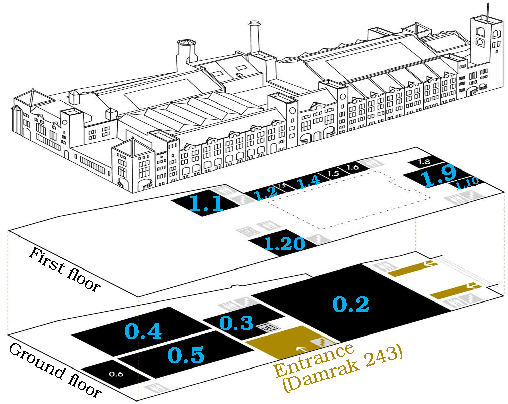
\includegraphics[width=\textwidth]{images/BvB-plan-3D-85mm-x-68mm.pdf}%
 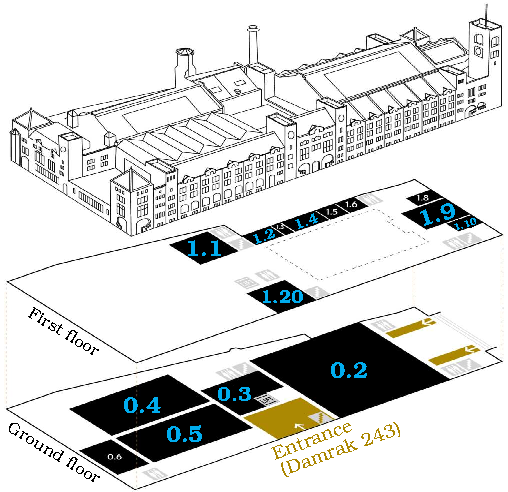
\includegraphics[width=\textwidth]{images/BvB-plan-3D-85mm-x-83mm.pdf}%

%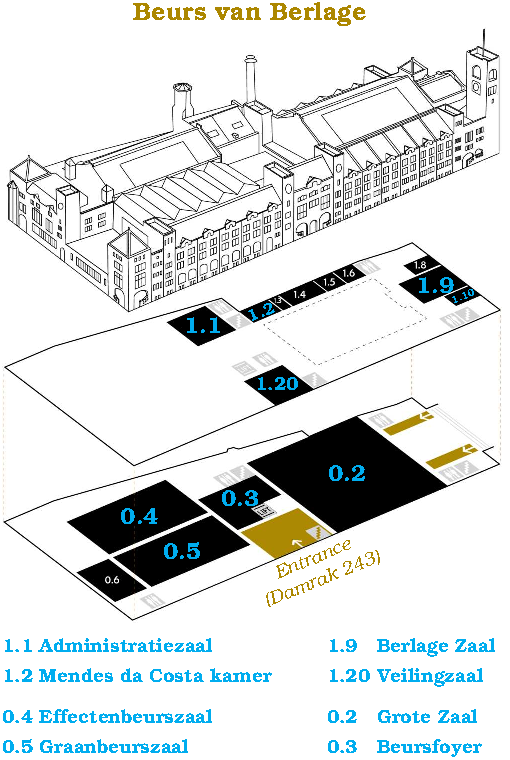
\includegraphics[width=\textwidth]{images/BvB-plan-3D-85mm-x-128mm.pdf}%

%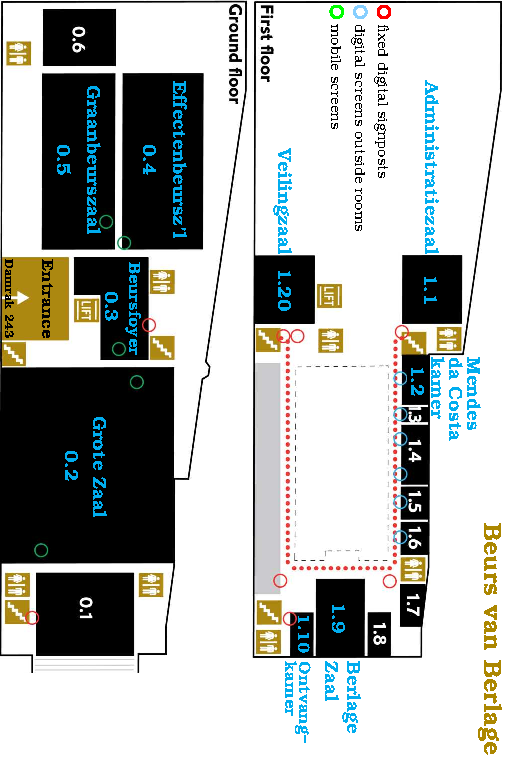
\includegraphics[width=\textwidth]{images/BvB-plan-2D-85mm-x-128mm-left.pdf}%

~
\vfill
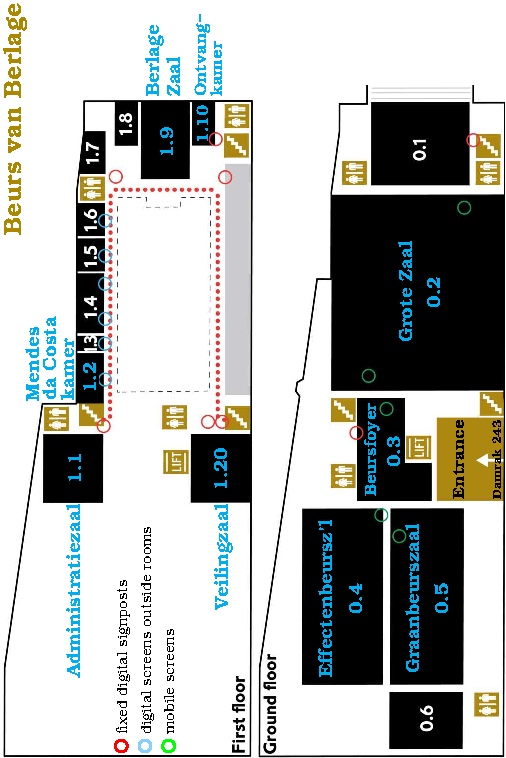
\includegraphics[width=.95\textwidth]{images/BvB-plan-2D-85mm-x-128mm-right.pdf}%


\section*{SIGMOD Reception - Van Gogh Museum}


\includegraphics[width=.5\textwidth]{images/reception/vangogh.jpeg}

The Van Gogh Museum maintains the world's largest collection of the works of the world's most popular artist - Vincent van Gogh (1853-1890), his paintings, drawings and letters, completed with the art of his contemporaries. Each year, it receives 1.6 million visitors, making it one of the 25 most popular museums in the world.

SIGMOD/PODS'2019 is proud to offer all participants registered to the main conference exclusive access to the Van Gogh Museum for the SIGMOD opening reception; on Tuesday July 2, 2019, from 20:30 until 23:00.
Your badge is our ticket into the museum, \textbf{you must bring it with you!}

We hereby like to thank \textbf{MonetDB} for sponsoring this event.

% 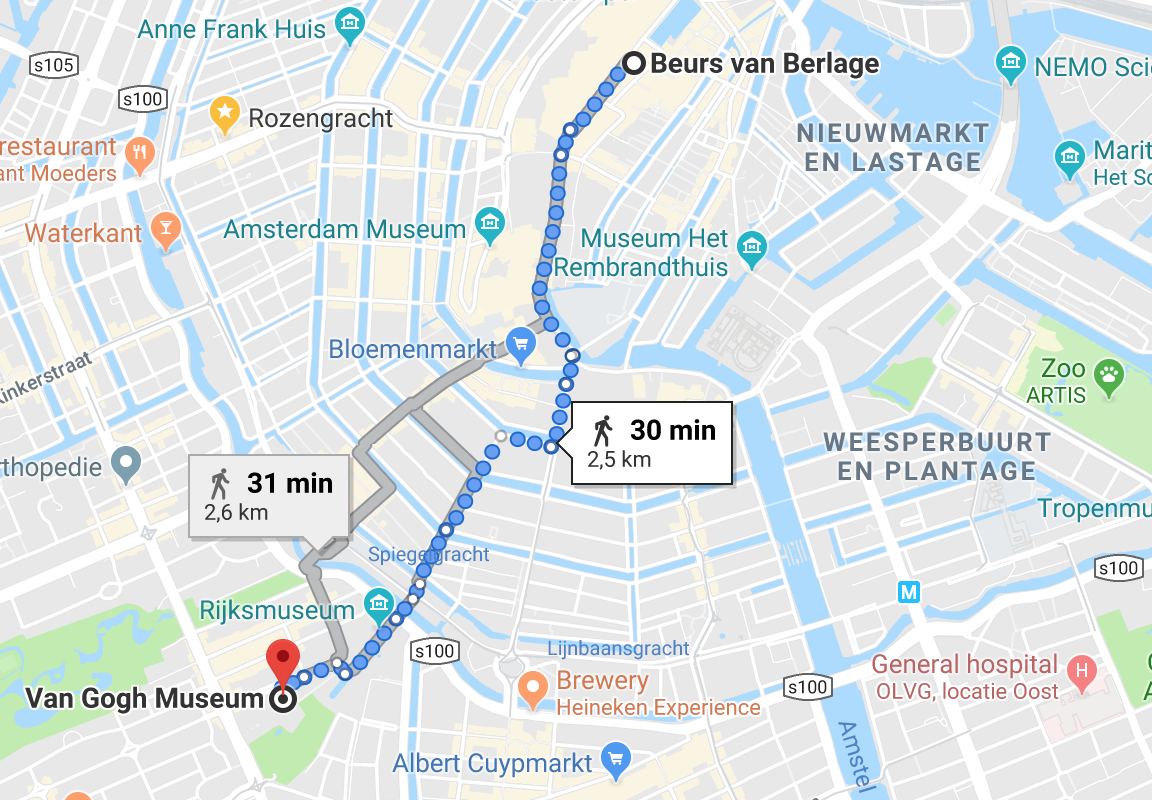
\includegraphics[width=.5\textwidth]{images/reception/berlage-vangogh.png}

There will be time to visit the museum; at the end of the walking route, back in the foyer, there will be drinks and snacks served. The reception food is intended to be dinner-replacing under moderate appetite.

Please note, again, the SIGMOD reception is on \textbf{Tuesday} evening (not Monday evening as usual in SIGMOD).

That day, the main program ends around 19:50; so participants have 40 minutes to get to the Museum, which is in the south center of Amsterdam (whereas the Beurs van Berlage conference center is in the middle of the center):

\begin{itemize}

\item Walking: \hfill 29 min (Instructions: \url{tiny.cc/m3kf7y})

\begin{minipage}{.9\textwidth}
\begin{wrapfigure}[3]{l}{1cm}
\vspace*{-1.2\baselineskip}%
\includegraphics[width=1cm]{images/reception/vangogh-walking.eps}
\end{wrapfigure}
Leave the venue taking a left and walk south to Dam square, and straight on into Rokin. Continue walking on Rokin until its end, at Munt tower. Continue into Muntplein which becomes Vijzelstraat until crossing the first main canal bridge, after which you take a right onto Herengracht. At the first opportunity you then go left into the Nieuwe Spiegelgracht. Continue this one straight, crossing no less than 4 canals (Prinsen, Keizers, Lijnbaans, Singel). The road passes under the Rijksmuseum; and continuing straight you will hit the Van Gogh museum.
\end{minipage}

\item Cycling: \hfill 10 min (Instructions: \url{tiny.cc/m3kf7y})

\begin{minipage}{.9\textwidth}
\begin{wrapfigure}[3]{l}{1cm}
\vspace*{-1.2\baselineskip}%
\includegraphics[width=1cm]{images/reception/vangogh-walking.eps}
\end{wrapfigure}
You can follow the same route as with walking, above. Use the bicycle path (or street), though, rather than the pedestrian sidewalk.
\end{minipage}

\item Metro 52: \hfill 19 min (Instructions: \url{tiny.cc/vmkf7y})

\begin{minipage}{.9\textwidth}
\begin{wrapfigure}[3]{l}{1cm}
\vspace*{-1.2\baselineskip}%
\includegraphics[width=1cm]{images/reception/vangogh-metro.eps}
\end{wrapfigure}
Leave the venue taking a left and walk south to Dam square, and straight on into Rokin. Earlier than indicated on the Google map, right after leaving Dam Square, there is a metro entrance, in front of Hudon's Bay. Metro 52 is Amsterdam's newest metro and its stations are quite beautiful. Take the metro in southward direction (Station Zuid) and exit at the very first stop (Vijzelgracht). Outside, take a right at the big roundabout into Weteringsschans. At the first main crossing, take a left onto the Museumbrug (bridge). The road passes under the Rijksmuseum; and continuing straight you will hit the Van Gogh museum.
~\hspace*{\fill}\mbox{\emph{(Involves ca.\ 16 min walking.)}}
\end{minipage}

\pagebreak
\item Tram 24: \hfill 20 min (Instructions: \url{tiny.cc/vm6i7y})

\begin{minipage}{.9\textwidth}
\begin{wrapfigure}[3]{l}{1cm}
\vspace*{-1.2\baselineskip}%

\includegraphics[width=1cm]{images/reception/vangogh-tram-24.png}
\end{wrapfigure}
Leave the venue taking a left and walk south to Dam square. At the tram stop just before Dam square, take tram 24 in southward direction (VU medisch centrum). At the 4th stop (Marie Heinekenplein), just after passing the former Heineken Brewery building (now hosting the "Heineken Experience") leave the tram, walk a few steps back and turn left (westward) into Eerste Jacob van Campenstraat. Continue staight on westward, crossing a canal, until Museum Plein (Square) opens in front of you. On your left-hand side, across the grass field, you see the new entrance hall of the Van Gogh Museum.
~\hspace*{\fill}\mbox{\emph{(Involves ca.\ 12 min walking.)}}
\end{minipage}

\item Tram 2/12: \hfill 17 min (Instructions: \url{tiny.cc/fdkf7y})

\begin{minipage}{.9\textwidth}
\begin{wrapfigure}[3]{l}{1cm}
\vspace*{-1.2\baselineskip}%
\includegraphics[width=1cm]{images/reception/vangogh-tram.eps}
\end{wrapfigure}
Leave the venue taking a left and walk south to Dam square. At Dam square, go right and walk in between the Palace and the Church to the Nieuwezijds Voorburgwal. There is a tram stop there, where you can either take tram 2 or 12  -- they take the same route up until its 7th stop, Van Baerlestraat, where you exit. The tram will just have passed the Van Gogh museum (it is on the left side seen from the tram), so you have to walk back a bit and cross the street.
~\hspace*{\fill}\mbox{\emph{(Involves ca.\ 6 min walking.)}}
\end{minipage}

\end{itemize}

You can of course also try to take a taxi or Uber, but taxi drivers will not be enthusiastically accepting such short trips; doing so will also not be much faster than the other options (or even slower, when stuck in a traffic jam) and quite expensive. Using a car is only recommended if walking is impossible for you. If you just want to minimize walking distance, the last option above (Tram 2 or 12) involves least walking.

\clearpage
% start even (left) page
% such that the 3x two schedule pages/days are adjacent to / facing eachother
\ifodd\value{page}\hbox{}\newpage\fi

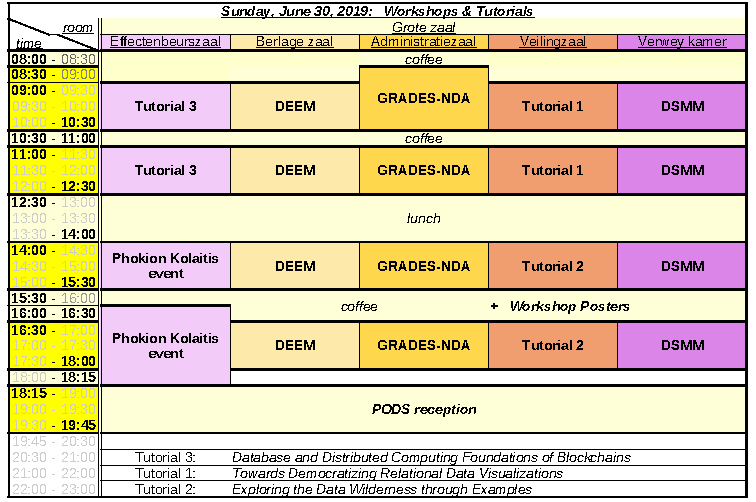
\includegraphics[angle=90,width=\textwidth]{schedule/p1.pdf}%

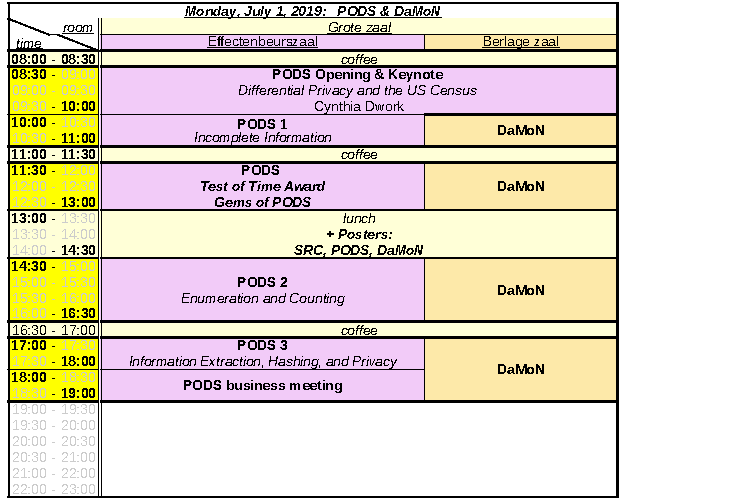
\includegraphics[angle=90,width=\textwidth]{schedule/p2.pdf}%

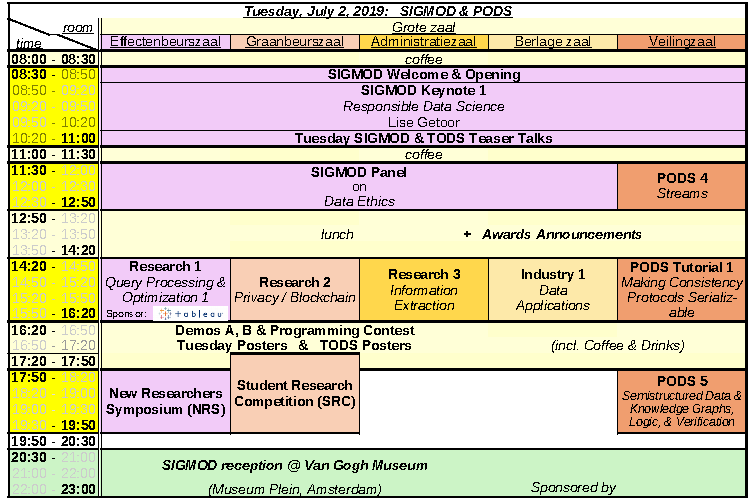
\includegraphics[angle=90,width=\textwidth]{schedule/p3.pdf}%


\includegraphics[angle=90,width=\textwidth]{schedule/p4.pdf}%


\includegraphics[angle=90,width=\textwidth]{schedule/p5.pdf}%

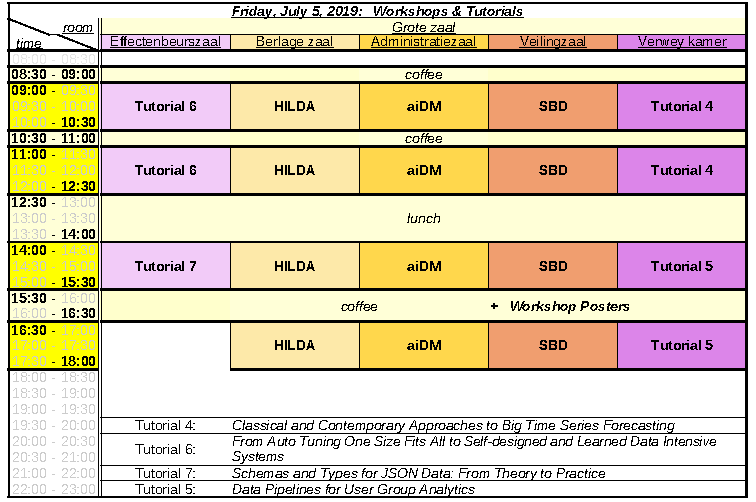
\includegraphics[angle=90,width=\textwidth]{schedule/p6.pdf}%

\slotheading{Sunday 06/30 08:00-09:00}

\sessionname{Coffee + Light Breakfast}{Coffee + Light Breakfast}\\
\sessiontimeloc{Sunday 08:00-09:00}{Grote Zaal}
\sessionlocation{Grote Zaal}

\sessionsep{}
\slotheading{Sunday 06/30 09:00-10:30}

\sessionname{Tutorial 1: part 1}{Tutorial 1: part 1}\\
\sessiontimeloc{Sunday 09:00-10:30}{Veilingzaal}
\sessionlocation{Veilingzaal}

\sessionsep{}
\papertitle{Towards Democratizing Relational Data Visualization}{https://doi.org/10.1145/3299869.3323598}
\paperauthors{Nan Tang (Qatar Foundation), Eugene Wu (Columbia University), Guoliang Li (Tsinghua University)}

\sessionname{GRADES-NDA Workshop: Session 1 (starts 08:30)}{GRADES-NDA 2019: Session 1 (starts 08:30)}\\
\sessiontimeloc{Sunday 09:00-10:30}{Administratiezaal}
\sessionlocation{Administratiezaal}

\sessionsep{}
\papertitle{GRADES-NDA 2019: Joint International Workshop on Graph Data Management Experiences \& Systems and Network Data Analytics}{https://sites.google.com/site/gradesnda2019/}
\paperauthors{Akhil Arora (EPFL), Arnab Bhattacharya (IIT Kanpur), George Fletcher (TU Eindhoven)}

\sessionname{DEEM Workshop: Session 1}{DEEM 2019: Session 1}\\
\sessiontimeloc{Sunday 09:00-10:30}{Berlage Zaal}
\sessionlocation{Berlage Zaal}

\sessionsep{}
\papertitle{DEEM 2019: Workshop on Data Management for End-to-End Machine Learning}{http://deem-workshop.org/}
\paperauthors{Sebastian Schelter (New York University), Neoklis Polyzotis (Google), Manasi Vartak (Massachusetts Institute of Technology), Stephan Seufert (Amazon Research)}

\sessionname{Tutorial 3: part 1}{Tutorial 3: part 1}\\
\sessiontimeloc{Sunday 09:00-10:30}{Effectenbeurszaal}
\sessionlocation{Effectenbeurszaal}

\sessionsep{}
\papertitle{Database and Distributed Computing Foundations of Blockchains}{https://doi.org/10.1145/3299869.3323667}
\paperauthors{Sujaya Maiyya (University of California, Santa Barbara), Victor Zakhary (University of California, Santa Barbara), Mohammad Javad Amiri (University of California, Santa Barbara), Divyakant Agrawal (University of California, Santa Barbara), Amr El Abbadi (University of California, Santa Barbara)}

\sessionname{DSMM Workshop: Session 1}{DSMM 2019: Session 1}\\
\sessiontimeloc{Sunday 09:00-10:30}{Mendes da Costa Kamer}
\sessionlocation{Mendes da Costa Kamer}

\sessionsep{}
\papertitle{DSMM 2019: the 5th Workshop on Data Science for Macro-modeling with Financial and Economic Datasets}{https://wiki.umiacs.umd.edu/clip/datascience/index.php/DSMM:_Data_Science_for_Macro-Modeling_with_Financial_and_Economic_Datasets}
\paperauthors{Douglas Burdick (IBM Almaden Research Center), Rajasekar Krishnamurthy (IBM T. J. Watson Research Center), Louiqa Raschid (University of Maryland)}

\slotheading{Sunday 06/30 10:30-11:00}

\sessionname{Coffee}{Coffee}\\
\sessiontimeloc{Sunday 10:30-11:00}{Grote Zaal}
\sessionlocation{Grote Zaal}

\sessionsep{}
\slotheading{Sunday 06/30 11:00-12:30}

\sessionname{Tutorial 1: part 2}{Tutorial 1: part 2}\\
\sessiontimeloc{Sunday 11:00-12:30}{Veilingzaal}
\sessionlocation{Veilingzaal}

\sessionsep{}
\papertitle{Towards Democratizing Relational Data Visualization}{https://doi.org/10.1145/3299869.3323598}
\paperauthors{Nan Tang (Qatar Foundation), Eugene Wu (Columbia University), Guoliang Li (Tsinghua University)}

\sessionname{GRADES-NDA Workshop: Session 2}{GRADES-NDA 2019: Session 2}\\
\sessiontimeloc{Sunday 11:00-12:30}{Administratiezaal}
\sessionlocation{Administratiezaal}

\sessionsep{}
\papertitle{GRADES-NDA 2019: Joint International Workshop on Graph Data Management Experiences \& Systems and Network Data Analytics}{https://sites.google.com/site/gradesnda2019/}
\paperauthors{Akhil Arora (EPFL), Arnab Bhattacharya (IIT Kanpur), George Fletcher (TU Eindhoven)}

\sessionname{DEEM Workshop: Session 2}{DEEM 2019: Session 2}\\
\sessiontimeloc{Sunday 11:00-12:30}{Berlage Zaal}
\sessionlocation{Berlage Zaal}

\sessionsep{}
\papertitle{DEEM 2019: Workshop on Data Management for End-to-End Machine Learning}{http://deem-workshop.org/}
\paperauthors{Sebastian Schelter (New York University), Neoklis Polyzotis (Google), Manasi Vartak (Massachusetts Institute of Technology), Stephan Seufert (Amazon Research)}

\sessionname{Tutorial 3: part 2}{Tutorial 3: part 2}\\
\sessiontimeloc{Sunday 11:00-12:30}{Effectenbeurszaal}
\sessionlocation{Effectenbeurszaal}

\sessionsep{}
\papertitle{Database and Distributed Computing Foundations of Blockchains}{https://doi.org/10.1145/3299869.3323667}
\paperauthors{Sujaya Maiyya (University of California, Santa Barbara), Victor Zakhary (University of California, Santa Barbara), Mohammad Javad Amiri (University of California, Santa Barbara), Divyakant Agrawal (University of California, Santa Barbara), Amr El Abbadi (University of California, Santa Barbara)}

\sessionname{DSMM Workshop: Session 2}{DSMM 2019: Session 2}\\
\sessiontimeloc{Sunday 11:00-12:30}{Mendes da Costa Kamer}
\sessionlocation{Mendes da Costa Kamer}

\sessionsep{}
\papertitle{DSMM 2019: the 5th Workshop on Data Science for Macro-modeling with Financial and Economic Datasets}{https://wiki.umiacs.umd.edu/clip/datascience/index.php/DSMM:_Data_Science_for_Macro-Modeling_with_Financial_and_Economic_Datasets}
\paperauthors{Douglas Burdick (IBM Almaden Research Center), Rajasekar Krishnamurthy (IBM T. J. Watson Research Center), Louiqa Raschid (University of Maryland)}

\slotheading{Sunday 06/30 12:30-14:00}

\sessionname{Lunch}{Lunch}\\
\sessiontimeloc{Sunday 12:30-14:00}{Grote Zaal}
\sessionlocation{Grote Zaal}

\sessionsep{}
\slotheading{Sunday 06/30 14:00-15:30}

\sessionname{Tutorial 2: part 1}{Tutorial 2: part 1}\\
\sessiontimeloc{Sunday 14:00-15:30}{Veilingzaal}
\sessionlocation{Veilingzaal}

\sessionsep{}
\papertitle{Exploring the Data Wilderness through Examples}{https://doi.org/10.1145/3299869.3323669}
\paperauthors{Davide Mottin (Aarhus University), Matteo Lissandrini (Aalborg University), Yannis Velegrakis (Utrecht University), Themis Palpanas (Paris Descartes University)}

\sessionname{GRADES-NDA Workshop: Session 3}{GRADES-NDA 2019: Session 3}\\
\sessiontimeloc{Sunday 14:00-15:30}{Administratiezaal}
\sessionlocation{Administratiezaal}

\sessionsep{}
\papertitle{GRADES-NDA 2019: Joint International Workshop on Graph Data Management Experiences \& Systems and Network Data Analytics}{https://sites.google.com/site/gradesnda2019/}
\paperauthors{Akhil Arora (EPFL), Arnab Bhattacharya (IIT Kanpur), George Fletcher (TU Eindhoven)}

\sessionname{DEEM Workshop: Session 3}{DEEM 2019: Session 3}\\
\sessiontimeloc{Sunday 14:00-15:30}{Berlage Zaal}
\sessionlocation{Berlage Zaal}

\sessionsep{}
\papertitle{DEEM 2019: Workshop on Data Management for End-to-End Machine Learning}{http://deem-workshop.org/}
\paperauthors{Sebastian Schelter (New York University), Neoklis Polyzotis (Google), Manasi Vartak (Massachusetts Institute of Technology), Stephan Seufert (Amazon Research)}

\sessionname{PODS: Phokion Kolaitis Special Event: part 1}{Phokion Kolaitis Special Event: part 1}\\
\sessiontimeloc{Sunday 14:00-15:30}{Effectenbeurszaal}
\sessionlocation{Effectenbeurszaal}

\sessionsep{}
\papertitle{Phokion Kolaitis Special Event}{https://sigmod2019.org/Kolaitis_Event}
\paperauthors{Georg Gottlob (University of Oxford), Wang-Chiew Tan (Megagon Labs)}

\sessionname{DSMM Workshop: Session 3}{DSMM 2019: Session 3}\\
\sessiontimeloc{Sunday 14:00-15:30}{Mendes da Costa Kamer}
\sessionlocation{Mendes da Costa Kamer}

\sessionsep{}
\papertitle{DSMM 2019: the 5th Workshop on Data Science for Macro-modeling with Financial and Economic Datasets}{https://wiki.umiacs.umd.edu/clip/datascience/index.php/DSMM:_Data_Science_for_Macro-Modeling_with_Financial_and_Economic_Datasets}
\paperauthors{Douglas Burdick (IBM Almaden Research Center), Rajasekar Krishnamurthy (IBM T. J. Watson Research Center), Louiqa Raschid (University of Maryland)}

\slotheading{Sunday 06/30 15:30-16:30}

\sessionname{Coffee + Workshop Posters}{Coffee + Workshop Posters}\\
\sessiontimeloc{Sunday 15:30-16:30}{Grote Zaal}
\sessionlocation{Grote Zaal}

\sessionsep{}
\slotheading{Sunday 06/30 16:30-18:00}

\sessionname{Tutorial 2: part 2}{Tutorial 2: part 2}\\
\sessiontimeloc{Sunday 16:30-18:00}{Veilingzaal}
\sessionlocation{Veilingzaal}

\sessionsep{}
\papertitle{Exploring the Data Wilderness through Examples}{https://doi.org/10.1145/3299869.3323669}
\paperauthors{Davide Mottin (Aarhus University), Matteo Lissandrini (Aalborg University), Yannis Velegrakis (Utrecht University), Themis Palpanas (Paris Descartes University)}

\sessionname{GRADES-NDA Workshop: Session 4}{GRADES-NDA 2019: Session 4}\\
\sessiontimeloc{Sunday 16:30-18:00}{Administratiezaal}
\sessionlocation{Administratiezaal}

\sessionsep{}
\papertitle{GRADES-NDA 2019: Joint International Workshop on Graph Data Management Experiences \& Systems and Network Data Analytics}{https://sites.google.com/site/gradesnda2019/}
\paperauthors{Akhil Arora (EPFL), Arnab Bhattacharya (IIT Kanpur), George Fletcher (TU Eindhoven)}

\sessionname{DEEM Workshop: Session 4}{DEEM 2019: Session 4}\\
\sessiontimeloc{Sunday 16:30-18:00}{Berlage Zaal}
\sessionlocation{Berlage Zaal}

\sessionsep{}
\papertitle{DEEM 2019: Workshop on Data Management for End-to-End Machine Learning}{http://deem-workshop.org/}
\paperauthors{Sebastian Schelter (New York University), Neoklis Polyzotis (Google), Manasi Vartak (Massachusetts Institute of Technology), Stephan Seufert (Amazon Research)}

\sessionname{PODS: Phokion Kolaitis Special Event: part 2 (16:00-18:15)}{Phokion Kolaitis Special Event: part 2 (16:00-18:15)}\\
\sessiontimeloc{Sunday 16:30-18:00}{Effectenbeurszaal}
\sessionlocation{Effectenbeurszaal}

\sessionsep{}
\papertitle{Phokion Kolaitis Special Event}{https://sigmod2019.org/Kolaitis_Event}
\paperauthors{Georg Gottlob (University of Oxford), Wang-Chiew Tan (Megagon Labs)}

\sessionname{DSMM Workshop: Session 4}{DSMM 2019: Session 4}\\
\sessiontimeloc{Sunday 16:30-18:00}{Mendes da Costa Kamer}
\sessionlocation{Mendes da Costa Kamer}

\sessionsep{}
\papertitle{DSMM 2019: the 5th Workshop on Data Science for Macro-modeling with Financial and Economic Datasets}{https://wiki.umiacs.umd.edu/clip/datascience/index.php/DSMM:_Data_Science_for_Macro-Modeling_with_Financial_and_Economic_Datasets}
\paperauthors{Douglas Burdick (IBM Almaden Research Center), Rajasekar Krishnamurthy (IBM T. J. Watson Research Center), Louiqa Raschid (University of Maryland)}

\slotheading{Sunday 06/30 18:15-19:45}

\sessionname{PODS Reception}{PODS Reception}\\
\sessiontimeloc{Sunday 18:15-19:45}{Grote Zaal}
\sessionlocation{Grote Zaal}

\sessionsep{}
\slotheading{Monday 01/07 08:00-08:30}

\sessionname{Coffee + Light Breakfast:2}{Coffee + Light Breakfast}\\
\sessiontimeloc{Monday 08:00-08:30}{Grote Zaal}
\sessionlocation{Grote Zaal}

\sessionsep{}
\slotheading{Monday 01/07 08:30-10:00}

\sessionname{PODS Opening + Keynote}{PODS Opening \& Keynote}\\
\sessiontimeloc{Monday 08:30-10:00}{Effectenbeurszaal}
\sessionlocation{Effectenbeurszaal}

\sessionchair{Christoph Koch}

\sessionsep{}
\papertitle{Differential Privacy and the US Census}{https://doi.org/10.1145/3294052.3322188}
\paperauthors{Cynthia Dwork (Harvard University)}

\slotheading{Monday 01/07 10:00-11:00}

\sessionname{PODS 1}{PODS 1: Incomplete Information}\\
\sessiontimeloc{Monday 10:00-11:00}{Effectenbeurszaal}
\sessionlocation{Effectenbeurszaal}

\sessionchair{Pierre Senellart}

\sessionsep{}
\papertitle{Regularizing Conjunctive Features for Classification}{https://doi.org/10.1145/3294052.3319680}
\paperauthors{Pablo Barceló (University of Chile \& IMFD Chile), Alexander Baumgartner (University of Chile \& RISC, Johannes Kepler University), Victor Dalmau (Universitat Pompeu Fabra), Benny Kimelfeld (Technion)}

\papertitle{Probabilistic Databases with an Infinite Open-World Assumption}{https://doi.org/10.1145/3294052.3319681}
\paperauthors{Martin Grohe (RWTH Aachen University), Peter Lindner (RWTH Aachen University)}

\papertitle{Query Evaluation in Election Databases}{https://doi.org/10.1145/3294052.3319692}
\paperauthors{Benny Kimelfeld (Technion), Phokion Kolaitis (University of California, Santa Cruz \& IBM Research-Almaden), Muhammad Tibi (Technion)}

\sessionname{DaMoN Workshop: Session 1}{DaMoN 2019: Session 1}\\
\sessiontimeloc{Monday 10:00-11:00}{Berlage Zaal}
\sessionlocation{Berlage Zaal}

\sessionsep{}
\papertitle{DaMoN 2019: the 15th International Workshop on Data Management on New Hardware}{https://sites.google.com/view/damon2019/home-damon-2019}
\paperauthors{Thomas Neumann (Technische Universität München), Ken Salem (University of Waterloo)}

\slotheading{Monday 01/07 11:00-11:30}

\sessionname{Coffee:2}{Coffee}\\
\sessiontimeloc{Monday 11:00-11:30}{Grote Zaal}
\sessionlocation{Grote Zaal}

\sessionsep{}
\slotheading{Monday 01/07 11:30-13:00}

\sessionname{PODS Test-of-Time \& Gems}{Gems of PODS and Test-of-Time Award}\\
\sessiontimeloc{Monday 11:30-13:00}{Effectenbeurszaal}
\sessionlocation{Effectenbeurszaal}

\sessionchair{Benny Kimelfeld}

\sessionsep{}
\papertitle{A General Datalog-based Framework for Tractable Query Answering}{}
\paperauthors{Andrea Cali (Birkbeck College), Georg Gottlob (University of Oxford), Thomas Lukasiewicz (University of Oxford)}

\papertitle{Database Repairs and Consistent Query Answering: Origins and Further Developments}{https://doi.org/10.1145/3294052.3322190}
\paperauthors{Leopoldo Bertossi (RelationalAI \& Carleton University)}

\papertitle{Remembering the Probabilistic Analysis of Latent Semantic Indexing}{}
\paperauthors{Christos Papadimitriou (Columbia University)}

\sessionname{DaMoN Workshop: Session 2}{DaMoN 2019: Session 2}\\
\sessiontimeloc{Monday 11:30-13:00}{Berlage Zaal}
\sessionlocation{Berlage Zaal}

\sessionsep{}
\papertitle{DaMoN 2019: the 15th International Workshop on Data Management on New Hardware}{https://sites.google.com/view/damon2019/home-damon-2019}
\paperauthors{Thomas Neumann (Technische Universität München), Ken Salem (University of Waterloo)}

\slotheading{Monday 01/07 13:00-14:30}

\sessionname{Lunch + Posters (PODS, DaMoN, SIGMOD Student Research Competition)}{Lunch + Posters (PODS, DaMoN, SIGMOD Student Research Competition)}\\
\sessiontimeloc{Monday 13:00-14:30}{Grote Zaal}
\sessionlocation{Grote Zaal}

\sessionsep{}
\slotheading{Monday 01/07 14:30-16:30}

\sessionname{PODS 2}{PODS 2: Enumeration and Counting}\\
\sessiontimeloc{Monday 14:30-16:30}{Effectenbeurszaal}
\sessionlocation{Effectenbeurszaal}

\sessionchair{Dirk van Gucht}

\sessionsep{}
\papertitle{Efficient Logspace Classes for Enumeration, Counting, and Uniform Generation}{https://doi.org/10.1145/3294052.3319704}
\paperauthors{Marcelo Arenas (PUC \&amp; IMFD Chile), Luis Alberto Croquevielle (PUC \&amp; IMFD Chile), Rajesh Jayaram (Carnegie Mellon University), Cristian Riveros (PUC \&amp; IMFD Chile)}

\papertitle{Ranked Enumeration of Minimal Triangulations}{https://doi.org/10.1145/3294052.3319678}
\paperauthors{Noam Ravid (Technion), Dori Medini (Technion), Benny Kimelfeld (Technion)}

\papertitle{Enumeration on Trees with Tractable Combined Complexity and Efficient Updates}{https://doi.org/10.1145/3294052.3319702}
\paperauthors{Antoine Amarilli (LTCI, CNRS, Télécom ParisTech, Université Paris-Saclay), Pierre Bourhis (CRIStAL, CNRS UMR 9189, Inria Lille), Stefan Mengel (CNRS, CRIL UMR 8188), Matthias Niewerth (University of Bayreuth)}

\papertitle{Counting Database Repairs under Primary Keys Revisited}{https://doi.org/10.1145/3294052.3319703}
\paperauthors{Marco Calautti (University of Edinburgh), Marco Console (University of Edinburgh), Andreas Pieris (University of Edinburgh)}

\papertitle{The Complexity of Counting Cycles in the Adjacency List Streaming Model}{https://doi.org/10.1145/3294052.3319706}
\paperauthors{John Kallaugher (University of Texas at Austin), Andrew McGregor (University of Massachusetts Amherst), Eric Price (University of Texas at Austin), Sofya Vorotnikova (University of Massachusetts Amherst)}

\papertitle{On the Enumeration Complexity of Unions of Conjunctive Queries}{https://doi.org/10.1145/3294052.3319700}
\paperauthors{Nofar Carmeli (Technion), Markus Kröll (TU Wien)}

\sessionname{DaMoN Workshop: Session 3}{DaMoN 2019: Session 3}\\
\sessiontimeloc{Monday 14:30-16:30}{Berlage Zaal}
\sessionlocation{Berlage Zaal}

\sessionsep{}
\papertitle{DaMoN 2019: the 15th International Workshop on Data Management on New Hardware}{https://sites.google.com/view/damon2019/home-damon-2019}
\paperauthors{Thomas Neumann (Technische Universität München), Ken Salem (University of Waterloo)}

\slotheading{Monday 01/07 16:30-17:00}

\sessionname{Coffee:3}{Coffee}\\
\sessiontimeloc{Monday 16:30-17:00}{Grote Zaal}
\sessionlocation{Grote Zaal}

\sessionsep{}
\slotheading{Monday 01/07 17:00-18:00}

\sessionname{PODS 3}{PODS 3: Information Extraction, Hashing, and Privacy}\\
\sessiontimeloc{Monday 17:00-18:00}{Effectenbeurszaal}
\sessionlocation{Effectenbeurszaal}

\sessionchair{Yufei Tao}

\sessionsep{}
\papertitle{Split-Correctness in Information Extraction}{https://doi.org/10.1145/3294052.3319684}
\paperauthors{Johannes Doleschal (University of Bayreuth \& Hasselt University), Benny Kimelfeld (Technion), Wim Martens (University of Bayreuth), Yoav Nahshon (Technion), Frank Neven (Hasselt University \& Transnational University of Limburg)}

\papertitle{Robust Set Reconciliation via Locality Sensitive Hashing}{https://doi.org/10.1145/3294052.3319690}
\paperauthors{Michael Mitzenmacher (Harvard University), Tom Morgan (Harvard University \& Google)}

\papertitle{What Storage Access Privacy is Achievable with Small Overhead?}{https://doi.org/10.1145/3294052.3319695}
\paperauthors{Sarvar Patel (Google), Giuseppe Persiano (Google \& University of Salerno), Kevin Yeo (Google)}

\sessionname{DaMoN Workshop: Session 4}{DaMoN 2019: Session 4}\\
\sessiontimeloc{Monday 17:00-18:00}{Berlage Zaal}
\sessionlocation{Berlage Zaal}

\sessionsep{}
\papertitle{DaMoN 2019: the 15th International Workshop on Data Management on New Hardware}{https://sites.google.com/view/damon2019/home-damon-2019}
\paperauthors{Thomas Neumann (Technische Universität München), Ken Salem (University of Waterloo)}

\slotheading{Monday 01/07 18:00-19:00}

\sessionname{PODS Business Meeting}{PODS Business Meeting}\\
\sessiontimeloc{Monday 18:00-19:00}{Effectenbeurszaal}
\sessionlocation{Effectenbeurszaal}

\sessionsep{}
\sessionname{DaMoN Workshop: Session 4 (uninterrupted from 17:00)}{DaMoN 2019: Session 4 (uninterrupted from 17:00)}\\
\sessiontimeloc{Monday 18:00-19:00}{Berlage Zaal}
\sessionlocation{Berlage Zaal}

\sessionsep{}
\papertitle{DaMoN 2019: the 15th International Workshop on Data Management on New Hardware}{https://sites.google.com/view/damon2019/home-damon-2019}
\paperauthors{Thomas Neumann (Technische Universität München), Ken Salem (University of Waterloo)}

\slotheading{Tuesday 02/07 08:00-08:30}

\sessionname{Coffee + Light Breakfast:3}{Coffee + Light Breakfast}\\
\sessiontimeloc{Tuesday 08:00-08:30}{Grote Zaal}
\sessionlocation{Grote Zaal}

\sessionsep{}
\slotheading{Tuesday 02/07 08:30-10:20}

\sessionname{SIGMOD Welcome + Keynote}{SIGMOD Welcome + Keynote}\\
\sessiontimeloc{Tuesday 08:30-10:20}{Effectenbeurszaal}
\sessionlocation{Effectenbeurszaal}

\sessionchair{Peter Boncz}

\sessionsep{}
\papertitle{Responsible Data Science}{https://doi.org/10.1145/3299869.3314117}
\paperauthors{Lise Getoor (University of California, Santa Cruz)}

\slotheading{Tuesday 02/07 10:20-11:00}

\sessionname{SIGMOD Teaser Talks 1}{Teaser Talks for all Tuesday SIGMOD Research, Industrial Papers and TODS Posters}\\
\sessiontimeloc{Tuesday 10:20-11:00}{Effectenbeurszaal}
\sessionlocation{Effectenbeurszaal}

\sessionchair{Peter Boncz}

\sessionsep{}
\slotheading{Tuesday 02/07 11:00-11:30}

\sessionname{Coffee:4}{Coffee}\\
\sessiontimeloc{Tuesday 11:00-11:30}{Grote Zaal}
\sessionlocation{Grote Zaal}

\sessionsep{}
\slotheading{Tuesday 02/07 11:30-12:50}

\sessionname{SIGMOD Panel on Data Ethics}{SIGMOD Panel on Data Ethics}\\
\sessiontimeloc{Tuesday 11:30-12:50}{Effectenbeurszaal}
\sessionlocation{Effectenbeurszaal}

\sessionchair{H.V. Jagadish}

\sessionsep{}
\papertitle{The Responsibility Challenge for Data}{https://doi.org/10.1145/3299869.3314327}
\paperauthors{H. V. Jagadish (University of Michigan), Francesco Bonchi (ISI Foundation), Tina Eliassi-Rad (Northeastern University), Lise Getoor (University of California, Santa Cruz), Krishna Gummadi (Max Planck Institute for Software Systems), Julia Stoyanovich (New York University)}

\sessionname{PODS 4}{PODS 4: Streams}\\
\sessiontimeloc{Tuesday 11:30-12:50}{Veilingzaal}
\sessionlocation{Veilingzaal}

\sessionchair{Pablo Barceló}

\sessionsep{}
\papertitle{Tight Trade-offs for the Maximum k-Coverage Problem in the General Streaming Model}{https://doi.org/10.1145/3294052.3319691}
\paperauthors{Piotr Indyk (MIT), Ali Vakilian (MIT)}

\papertitle{Weighted Reservoir Sampling from Distributed Streams}{https://doi.org/10.1145/3294052.3319696}
\paperauthors{Rajesh Jayaram (Carnegie Mellon University), Gokarna Sharma (Kent State University), Srikanta Tirthapura (Iowa State University), David Woodruff (Carnegie Mellon University)}

\papertitle{Distributed and Streaming Linear Programming in Low Dimensions}{https://doi.org/10.1145/3294052.3319697}
\paperauthors{Sepehr Assadi (Princeton University), Nikolai Karpov (Indiana University), Qin Zhang (Indiana University)}

\papertitle{Better Sliding Window Algorithms to Maximize Subadditive and Diversity Objectives}{https://doi.org/10.1145/3294052.3319701}
\paperauthors{Michele Borassi (Google Research), Alessandro Epasto (Google Research), Silvio Lattanzi (Google Research), Sergei Vassilvitskii (Google Research), Morteza Zadimoghaddam (Google Research)}

\slotheading{Tuesday 02/07 12:50-14:20}

\sessionname{Lunch + SIGMOD Awards}{Lunch + SIGMOD Awards}\\
\sessiontimeloc{Tuesday 12:50-14:20}{Grote Zaal}
\sessionlocation{Grote Zaal}

\sessionsep{}
\slotheading{Tuesday 02/07 14:20-16:20}

\sessionname{SIGMOD Research 1}{SIGMOD Research 1: Query Processing \& Optimization 1 - sponsored by Tableau}\\
\sessiontimeloc{Tuesday 14:20-16:20}{Effectenbeurszaal}
\sessionlocation{Effectenbeurszaal}

\sessionchair{Wolfgang Lehner}

\sessionsep{}
\papertitle{Exact Cardinality Query Optimization with Bounded Execution Cost}{https://doi.org/10.1145/3299869.3300087}
\paperauthors{Immanuel Trummer (Cornell University)}

\papertitle{Pessimistic Cardinality Estimation}{https://doi.org/10.1145/3299869.3319894}
\paperauthors{Walter Cai (University of Washington), Magdalena Balazinska (University of Washington), Dan Suciu (University of Washington)}

\papertitle{Efficiently Searching In-Memory Sorted Arrays: Revenge of the Interpolation Search?}{https://doi.org/10.1145/3299869.3300075}
\paperauthors{Peter Van Sandt (University of Wisconsin, Madison), Yannis Chronis (University of Wisconsin, Madison), Jignesh Patel (University of Wisconsin, Madison)}

\papertitle{Iterative Query Processing based on Unified Optimization Techniques}{https://doi.org/10.1145/3299869.3324960}
\paperauthors{Kisung Park (Kyung Hee University), Hojin Seo (Kyung Hee University), Mostofa Rasel (Kyung Hee University), Young-Koo Lee (Kyung Hee University), Chanho Jeong (SAP Labs Korea), Sung Yeol Lee (SAP Labs Korea), Chungmin Lee (SAP Labs Korea), Dong-Hun Lee (SAP Labs Korea)}

\papertitle{Approximate Distinct Counts for Billions of Datasets}{https://doi.org/10.1145/3299869.3319897}
\paperauthors{Daniel Ting (Tableau Software)}

\papertitle{Cache-oblivious High-performance Similarity Join}{https://doi.org/10.1145/3299869.3319859}
\paperauthors{Martin Perdacher (University of Vienna), Claudia Plant (University of Vienna), Christian Böhm (Ludwig-Maximilians-Universität)}

\sessionname{SIGMOD Research 2}{SIGMOD Research 2: Privacy/Blockchain}\\
\sessiontimeloc{Tuesday 14:20-16:20}{Graanbeurszaal}
\sessionlocation{Graanbeurszaal}

\sessionchair{Raghav Kaushik}

\sessionsep{}
\papertitle{Blurring the Lines between Blockchains and Database Systems: the Case of Hyperledger Fabric}{https://doi.org/10.1145/3299869.3319883}
\paperauthors{Ankur Sharma (Saarland University), Felix Schuhknecht (Saarland University), Divya Agrawal (Saarland University), Jens Dittrich (Saarland University)}

\papertitle{Towards Scaling Blockchain Systems via Sharding}{https://doi.org/10.1145/3299869.3319889}
\paperauthors{Hung Dang (National University of Singapore), Tien Tuan Anh Dinh (National University of Singapore), Dumitrel Loghin (National University of Singapore), Ee-Chien Chang (National University of Singapore), Qian Lin (National University of Singapore), Beng Chin Ooi (National University of Singapore)}

\papertitle{vChain: Enabling Verifiable Boolean Range Queries over Blockchain Databases}{https://doi.org/10.1145/3299869.3300083}
\paperauthors{Cheng Xu (Hong Kong Baptist University), Ce Zhang (Hong Kong Baptist University), Jianliang Xu (Hong Kong Baptist University)}

\papertitle{Answering Multi-Dimensional Analytical Queries under Local Differential Privacy}{https://doi.org/10.1145/3299869.3319891}
\paperauthors{Tianhao Wang (Purdue University), Bolin Ding (Alibaba Group), Jingren Zhou (Alibaba Group), Cheng Hong (Alibaba Group), Zhicong Huang (Alibaba Group), Ninghui Li (Purdue University), Somesh Jha (University of Wisconsin, Madison)}

\papertitle{APEx: Accuracy-Aware Differentially Private Data Exploration}{https://doi.org/10.1145/3299869.3300092}
\paperauthors{Chang Ge (University of Waterloo), Xi He (University of Waterloo), Ihab Ilyas (University of Waterloo), Ashwin Machanavajjhala (Duke University)}

\papertitle{Active Sparse Mobile Crowd Sensing Based on Matrix Completion}{https://doi.org/10.1145/3299869.3319856}
\paperauthors{Kun Xie (Hunan University), Xiaocan Li (Hunan University), Xin Wang (Stony Brook University), Gaogang Xie (Institute of Computing Technology \& Chinese Academy of Sciences), Jigang Wen (Institute of Computing Technology \& Chinese Academy of Sciences), Dafang Zhang (Hunan University)}

\sessionname{SIGMOD Research 3}{SIGMOD Research 3: Information Extraction}\\
\sessiontimeloc{Tuesday 14:20-16:20}{Administratiezaal}
\sessionlocation{Administratiezaal}

\sessionchair{Guoliang Li}

\sessionsep{}
\papertitle{Autocompletion for Prefix-Abbreviated Input}{https://doi.org/10.1145/3299869.3319858}
\paperauthors{Sheng Hu (Nagoya University \& Kyoto University), Chuan Xiao (Nagoya University \& Osaka University), Jianbin Qin (Shenzhen University), Yoshiharu Ishikawa (Nagoya University), Qiang Ma (Kyoto University)}

\papertitle{Progressive Deep Web Crawling Through Keyword Queries For Data Enrichment}{https://doi.org/10.1145/3299869.3319899}
\paperauthors{Pei Wang (Simon Fraser University), Ryan Shea (Simon Fraser University), Jiannan Wang (Simon Fraser University), Eugene Wu (Columbia University)}

\papertitle{Visual Segmentation for Information Extraction from Heterogeneous Visually Rich Documents}{https://doi.org/10.1145/3299869.3319867}
\paperauthors{Ritesh Sarkhel (Ohio State University), Arnab Nandi (Ohio State University)}

\papertitle{RRR: Rank-Regret Representative}{https://doi.org/10.1145/3299869.3300080}
\paperauthors{Abolfazl Asudeh (University of Michigan), Azade Nazi (Google AI), Nan Zhang (Pennsylvania State University), Gautam Das (University of Texas at Arlington), H. V. Jagadish (University of Michigan)}

\papertitle{Strongly Truthful Interactive Regret Minimization}{https://doi.org/10.1145/3299869.3300068}
\paperauthors{Min Xie (Hong Kong University of Science and Technology), Raymond Chi-Wing Wong (Hong Kong University of Science and Technology), Ashwin Lall (Denison University)}

\papertitle{Verifying Text Summaries of Relational Data Sets}{https://doi.org/10.1145/3299869.3300074}
\paperauthors{Saehan Jo (Cornell University), Immanuel Trummer (Cornell University), Weicheng Yu (Cornell University), Xuezhi Wang (Google Research), Cong Yu (Google Research), Daniel Liu (Cornell University), Niyati Mehta (Cornell University)}

\sessionname{SIGMOD Industry 1}{SIGMOD Industry 1: Data Applications}\\
\sessiontimeloc{Tuesday 14:20-16:20}{Berlage Zaal}
\sessionlocation{Berlage Zaal}

\sessionchair{Marco Serafini}

\sessionsep{}
\papertitle{QuickInsights: Quick and Automatic Discovery of Insights from Multi-Dimensional Data}{https://doi.org/10.1145/3299869.3314037}
\paperauthors{Rui Ding (Microsoft Research), Shi Han (Microsoft Research), Yong Xu (Microsoft Research), Haidong Zhang (Microsoft Research), Dongmei Zhang (Microsoft Research)}

\papertitle{ExplainIt! – A Declarative Root-cause Analysis Engine for Time Series Data}{https://doi.org/10.1145/3299869.3314048}
\paperauthors{Vimalkumar Jeyakumar (Cisco Tetration Analytics), Omid Madani (Cisco Tetration Analytics), Ali Parandeh (Cisco Tetration Analytics), Ashutosh Kulshreshtha (Cisco Tetration Analytics), Weifei Zeng (Cisco Tetration Analytics), Navindra Yadav (Cisco Tetration Analytics)}

\papertitle{Automatically Generating Interesting Facts from Wikipedia Tables}{https://doi.org/10.1145/3299869.3314043}
\paperauthors{Flip Korn (Google Research), Xuezhi Wang (Google Research), You Wu (Google Research), Cong Yu (Google Research)}

\papertitle{Snorkel DryBell: A Case Study in Deploying Weak Supervision at Industrial Scale}{https://doi.org/10.1145/3299869.3314036}
\paperauthors{Stephen Bach (Brown University), Daniel Rodriguez (Google), Yintao Liu (Google), Chong Luo (Google), Haidong Shao (Google), Cassandra Xia (Google), Souvik Sen (Google), Alex Ratner (Stanford University), Braden Hancock (Stanford University), Houman Alborzi (Google), Rahul Kuchhal (Google), Chris Ré (Stanford University), Rob Malkin (Google)}

\papertitle{PS2: Parameter Server on Spark}{https://doi.org/10.1145/3299869.3314038}
\paperauthors{Zhipeng Zhang (Peking University \& Tencent Inc.), Bin Cui (Peking University), Yingxia Shao (Beijing University of Posts and Telecommunications), Lele Yu (Tencent Inc.), Jiawei Jiang (Tencent Inc.), Xupeng Miao (Peking University \& Tencent Inc.)}

\papertitle{Entity Matching Meets Data Science: A Progress Report from the Magellan Project}{https://doi.org/10.1145/3299869.3314042}
\paperauthors{Yash Govind (University of Wisconsin, Madison), Pradap Konda (University of Wisconsin, Madison), Paul Suganthan G.C. (Google), Philip Martinkus (University of Wisconsin, Madison), Palaniappan Nagarajan (University of Wisconsin, Madison), Aravind Soundararajan (University of Wisconsin, Madison), Han Li (University of Wisconsin, Madison), Sidharth Mudgal (University of Wisconsin, Madison), Jeff Ballard (University of Wisconsin, Madison), Haojun Zhang (University of Wisconsin, Madison), Adel Ardalan (University of Wisconsin, Madison), Sanjib Das (University of Wisconsin, Madison), Derek Paulsen (University of Wisconsin, Madison), Amanpreet Singh Saini (University of Wisconsin, Madison), Erik Paulson (University of Wisconsin, Madison), Youngchoon Park (Johnson Controls), Marshall Carter (American Family Insurance), Mingju Sun (American Family Insurance), Glenn Fung (American Family Insurance), AnHai Doan (University of Wisconsin, Madison)}

\sessionname{PODS Invited Tutorial 1}{PODS Invited Tutorial 1}\\
\sessiontimeloc{Tuesday 14:20-16:20}{Veilingzaal}
\sessionlocation{Veilingzaal}

\sessionchair{Pierre Bourhis}

\sessionsep{}
\papertitle{Making Consistency Protocols Serializable}{https://doi.org/10.1145/3294052.3322191}
\paperauthors{Alan Fekete (University of Sydney)}

\slotheading{Tuesday 02/07 16:20-17:50}

\sessionname{Poster \& Demo Reception 1}{Poster \& Demo Groups A and B}\\
\sessiontimeloc{Tuesday 16:20-17:50}{Grote Zaal}
\sessionlocation{Grote Zaal}

\sessionsep{}
\papertitle{One poster for each SIGMOD and PODS paper presented on Tuesday. Plus 5 Programming Contest demos.}{}
\paperauthors{}

\papertitle{Representations and Optimizations for Embedded Parallel Dataflow Languages}{https://doi.org/10.1145/3281629}
\paperauthors{Alexander Alexandrov (TU Berlin), Georgi Krastev (TU Berlin), Volker Markl (TU Berlin)}

\papertitle{A Survey of Spatial Crowdsourcing}{https://doi.org/10.1145/3291933}
\paperauthors{Srinivasa Raghavendra (Aalborg University), Bhuvan Gummidi (Aalborg University), Xike Xie (University of Science and Technology of China), Torben Bach Pedersen (Aalborg University)}

\papertitle{K-Regret Queries Using Multiplicative Utility Functions}{https://doi.org/10.1145/3230634}
\paperauthors{Jianzhong Qi (The University of Melbourne), Fei Zuo (The University of Melbourne), Hanan Samet (University of Maryland), Jia Cheng Yao (The University of Melbourne)}

\papertitle{Historic Moments Discovery in Sequence Data.}{https://doi.org/10.1145/3276975}
\paperauthors{Ran Bai (The Hong Kong Polytechnic University), Wing-Kai Hon (National Tsing Hua University, Taiwan), Eric Lo (Chinese University of Hong Kong), Zhian He (University of Hong Kong), Kenny Q. Zhu (Shanghai Jiao Tong University)}

\papertitle{FindYourFavorite: An Interactive System for Finding the User's Favorite Tuple in the Database}{https://doi.org/10.1145/3299869.3320215}
\paperauthors{Min Xie (Hong Kong University of Science and Technology), Tianwen Chen (Hong Kong University of Science and Technology), Raymond Chi-Wing Wong (Hong Kong University of Science and Technology)}

\papertitle{Large Scale Graph Mining with G-Miner}{https://doi.org/10.1145/3299869.3320219}
\paperauthors{Hongzhi Chen (The Chinese University of Hong Kong), Xiaoxi Wang (The Chinese University of Hong Kong), Chenghuan Huang (The Chinese University of Hong Kong), Juncheng Fang (The Chinese University of Hong Kong), Yifan Hou (The Chinese University of Hong Kong), Changji Li (The Chinese University of Hong Kong), James Cheng (The Chinese University of Hong Kong)}

\papertitle{ANMAT: Automatic Knowledge Discovery and Error Detection through Pattern Functional Dependencies}{https://doi.org/10.1145/3299869.3320209}
\paperauthors{Abdulhakim Qahtan (QCRI, HBKU), Nan Tang (QCRI, HBKU), Mourad Ouzzani (QCRI, HBKU), Yang Cao (University of Edinburgh), Michael Stonebraker (MIT)}

\papertitle{Estimating Cardinalities with Deep Sketches}{https://doi.org/10.1145/3299869.3320218}
\paperauthors{Andreas Kipf (Technische Universität München), Dimitri Vorona (Technische Universität München), Jonas Müller (Technische Universität München), Thomas Kipf (University of Amsterdam), Bernhard Radke (Technische Universität München), Viktor Leis (Technische Universität München), Peter Boncz (CWI), Thomas Neumann (Technische Universität München), Alfons Kemper (Technische Universität München)}

\papertitle{Unit Testing Data with Deequ}{https://doi.org/10.1145/3299869.3320210}
\paperauthors{Sebastian Schelter (Amazon Research), Felix Biessmann (Amazon Research), Dustin Lange (Amazon Research), Tammo Rukat (Amazon Research), Phillipp Schmidt (Amazon Research), Stephan Seufert (Amazon Research), Pierre Brunelle (Amazon Research), Andrey Taptunov (Amazon Research)}

\papertitle{DuckDB: an Embeddable Analytical Database}{https://doi.org/10.1145/3299869.3320212}
\paperauthors{Mark Raasveldt (CWI), Hannes Mühleisen (CWI)}

\papertitle{CLASH: A High-Level Abstraction for Optimized, Multi-Way Stream Joins over Apache Storm}{https://doi.org/10.1145/3299869.3320217}
\paperauthors{Manuel Dossinger (TU Kaiserslautern), Sebastian Michel (TU Kaiserslautern), Constantin Roudsarabi (TU Kaiserslautern)}

\papertitle{PgCuckoo: Laying Plan Eggs in PostgreSQL's Nest}{https://doi.org/10.1145/3299869.3320211}
\paperauthors{Denis Hirn (Universität Tübingen), Torsten Grust (Universität Tübingen)}

\papertitle{Demonstration of ModelarDB: Model-Based Management of Dimensional Time Series}{https://doi.org/10.1145/3299869.3320216}
\paperauthors{Søren Kejser Jensen (Aalborg University), Torben Bach Pedersen (Aalborg University), Christian Thomsen (Aalborg University)}

\papertitle{NEURON: Query Execution Plan Meets Natural Language Processing For Augmenting DB Education}{https://doi.org/10.1145/3299869.3320213}
\paperauthors{Siyuan Liu (Nanyang Technological University), Sourav Bhowmick (Nanyang Technological University), Wanlu Zhang (Nanyang Technological University), Shu Wang (Nanyang Technological University), Wanyi Huang (Nanyang Technological University), Shafiq Joty (Nanyang Technological University)}

\papertitle{PIClean: A Probabilistic and Interactive Data Cleaning System}{https://doi.org/10.1145/3299869.3320214}
\paperauthors{Zhuoran Yu (Georgia Institute of Technology), Xu Chu (Georgia Institute of Technology)}

\papertitle{Apollo: A Dataset Profiling and Operator Modeling System}{https://doi.org/10.1145/3299869.3320220}
\paperauthors{Tasos Bakogiannis (National Technical University of Athens), Ioannis Giannakopoulos (National Technical University of Athens), Dimitrios Tsoumakos (Ionian University), Nectarios Koziris (National Technical University of Athens)}

\papertitle{Pivotal Greenplum© for Kubernetes: Demonstration of Managing Greenplum Database on Kubernetes}{https://doi.org/10.1145/3299869.3320229}
\paperauthors{Jemish Patel (Pivotal Software Inc), Goutam Tadi (Pivotal Software Inc), Oz Basarir (Pivotal Software Inc), Lawrence Hamel (Pivotal Software Inc), David Sharp (Pivotal Software Inc), Fei Yang (Pivotal Software Inc), Xin Zhang (Pivotal Software Inc)}

\papertitle{Demonstration of SpeakQL: Speech-driven Multimodal Querying of Structured Data}{https://doi.org/10.1145/3299869.3320224}
\paperauthors{Vraj Shah (University of California, San Diego), Side Li (University of California, San Diego), Kevin Yang (University of California, San Diego), Arun Kumar (University of California, San Diego), Lawrence Saul (University of California, San Diego)}

\papertitle{Ratel: Interactive Analytics for Large Scale Trajectories}{https://doi.org/10.1145/3299869.3320222}
\paperauthors{Haoda Li (Tsinghua University), Guoliang Li (Tsinghua University), Jiayang Liu (Tsinghua University), Haitao Yuan (Tsinghua University), Haiquan Wang (Tsinghua University)}

\papertitle{MigCast: Putting a Price Tag on Data Model Evolution in NoSQL Data Stores}{https://doi.org/10.1145/3299869.3320223}
\paperauthors{Andrea Hillenbrand (Darmstadt University of Applied Sciences), Maksym Levchenko (Darmstadt University of Applied Sciences), Uta Störl (Darmstadt University of Applied Sciences), Stefanie Scherzinger (OTH Regensburg), Meike Klettke (University of Rostock)}

\papertitle{NeMeSys - A Showcase of Data Oriented Near Memory Graph Processing}{https://doi.org/10.1145/3299869.3320226}
\paperauthors{Alexander Krause (Technische Universität Dresden), Thomas Kissinger (Technische Universität Dresden), Dirk Habich (Technische Universität Dresden), Wolfgang Lehner (Technische Universität Dresden)}

\papertitle{Low-latency Spark Queries on Updatable Data}{https://doi.org/10.1145/3299869.3320227}
\paperauthors{Alexandru Uta (Vrije Universiteit Amsterdam), Bogdan Ghit (Databricks), Ankur Dave (University of California, Berkeley), Peter Boncz (CWI)}

\papertitle{Demonstration of Nimbus: Model-based Pricing for Machine Learning in a Data Marketplace}{https://doi.org/10.1145/3299869.3320231}
\paperauthors{Lingjiao Chen (University of Wisconsin, Madison), Hongyi Wang (University of Wisconsin, Madison), Leshang Chen (University of Pennsylvania), Paraschos Koutris (University of Wisconsin, Madison), Arun Kumar (University of California, San Diego)}

\papertitle{Capturing and Querying Structural Provenance in Spark with Pebble}{https://doi.org/10.1145/3299869.3320225}
\paperauthors{Ralf Diestelkämper (Universität Stuttgart), Melanie Herschel (Universität Stuttgart)}

\papertitle{SVQ: Streaming Video Queries}{https://doi.org/10.1145/3299869.3320230}
\paperauthors{Ioannis Xarchakos (University of Toronto), Nick Koudas (University of Toronto)}

\papertitle{GraphWrangler: An Interactive Graph View on Relational Data}{https://doi.org/10.1145/3299869.3320232}
\paperauthors{Nafisa Anzum (University of Waterloo), Semih Salihoglu (University of Waterloo), Daniel Vogel (University of Waterloo)}

\papertitle{Coconut Palm: Static and Streaming Data Series Exploration Now in your Palm}{https://doi.org/10.1145/3299869.3320233}
\paperauthors{Haridimos Kondylakis (FORTH-ICS), Niv Dayan (Harvard University), Kostas Zoumpatianos (Harvard University), Themis Palpanas (Paris Descartes University)}

\papertitle{Natural Language Querying of Complex Business Intelligence Queries}{https://doi.org/10.1145/3299869.3320248}
\paperauthors{Jaydeep Sen (IBM Research AI), Fatma Ozcan (IBM Research AI), Abdul Quamar (IBM Research AI), Greg Stager (IBM Canada), Ashish Mittal (IBM Research AI), Manasa Jammi (IBM Research AI), Chuan Lei (IBM Research AI), Diptikalyan Saha (IBM Research AI), Karthik Sankaranarayanan (IBM Research AI)}

\slotheading{Tuesday 02/07 17:50-19:50}

\sessionname{New Researcher Symposium}{New Researcher Symposium}\\
\sessiontimeloc{Tuesday 17:50-19:50}{Effectenbeurszaal}
\sessionlocation{Effectenbeurszaal}

\sessionsep{}
\papertitle{Publication Strategies for New Researchers: intro by the organizers}{https://http://sigmod2019.org/new_researchers_symp}
\paperauthors{Katja Hose (Aalborg University), Spyros Blanas (Ohio State University)}

\papertitle{title unknown}{http://adityagp.net}
\paperauthors{Aditya Parameswaran (University of California, Berkeley)}

\papertitle{title unknown}{http://azza.azurewebsites.net/}
\paperauthors{Azza Abouzied (New York University, Abu Dhabi)}

\papertitle{title unknown}{https://stratos.seas.harvard.edu/}
\paperauthors{Stratos Idreos (Harvard University)}

\papertitle{title unknown}{http://lig-membres.imag.fr/amery/}
\paperauthors{Sihem Amer-Yahia (CNRS)}

\papertitle{title unknown}{https://web.eecs.umich.edu/~jag/}
\paperauthors{H.V. Jagadish (University of Michigan)}

\sessionname{Student Research Competition (starts 17:20)}{Student Research Competition}\\
\sessiontimeloc{Tuesday 17:50-19:50}{Graanbeurszaal}
\sessionlocation{Graanbeurszaal}

\sessionsep{}
\papertitle{SpeakQL: Towards Speech-driven Multimodal Querying}{https://doi.org/10.1145/3299869.3323596}
\paperauthors{Vraj Shah (University of California, San Diego)}

\papertitle{Fingerprints for Compressed Columnar Data Search}{https://doi.org/10.1145/3299869.3323597}
\paperauthors{Carmen Kwan (University of Waterloo)}

\papertitle{CAvSAT: A System for Query Answering over Inconsistent Databases}{https://doi.org/10.1145/3299869.3323598}
\paperauthors{Akhil Dixit (University of California, Santa Cruz)}

\papertitle{Scalable Reservoir Sampling on Many-Core CPUs}{https://doi.org/10.1145/3299869.3323667}
\paperauthors{Altan Birler (Technische Universität München)}

\papertitle{LSM-Trees and B-Trees: The Best of Both Worlds}{https://doi.org/10.1145/3299869.3323669}
\paperauthors{Varun Jain (Harvard University), James Lennon (Harvard University), Harshita Gupta (Harvard University)}

\papertitle{Generating Selective Filters for Access Method and PhysicalDesign Evaluation}{https://doi.org/10.1145/3299869.3314032}
\paperauthors{Pranav Subramaniam (University of Chicago)}

\papertitle{Interactive Visualization For Big Spatial Data}{https://doi.org/10.1145/3299869.3314034}
\paperauthors{Saheli Ghosh (University of California, Riverside)}

\papertitle{Learning to Generate Questions with Adaptive Copying Neural Networks}{https://doi.org/10.1145/3299869.3300100}
\paperauthors{Xinyuan Lu (Carleton University)}

\papertitle{Query-Driven Learning for Next Generation Predictive Modeling \& Analytics}{https://doi.org/10.1145/3299869.3300101}
\paperauthors{Fotis Savva (University of Glasgow)}

\papertitle{Answering Range Queries Under Local Differential Privacy}{https://doi.org/10.1145/3299869.3300102}
\paperauthors{Tejas Kulkarni (University of Warwick)}

\papertitle{Helios: An Adaptive and Query Workload-driven Partitioning Framework for Distributed Graph Stores}{https://doi.org/10.1145/3299869.3300103}
\paperauthors{Ali Davoudian (Carleton University)}

\papertitle{Deep Query Optimization}{https://doi.org/10.1145/3299869.3300104}
\paperauthors{Tin Vu (University of California, Riverside)}

\papertitle{Bootstrapping an End-to-End Natural Language Interface for Databases}{https://doi.org/10.1145/3299869.3300105}
\paperauthors{Nathaniel Weir (Brown University), Prasetya Utama (TU Darmstadt)}

\papertitle{Recommending Deployment Strategies in Crowdsourcing Platforms}{https://doi.org/10.1145/3299869.3300106}
\paperauthors{Dong Wei (New Jersey Institute of Technology)}

\papertitle{Towards Understanding Data Analysis Workflows using a Large Notebook Corpus}{https://doi.org/10.1145/3299869.3300107}
\paperauthors{Mohammed Suhail Rehman (University of Chicago)}

\papertitle{Arachnid: Generalized Visual Data Cleaning}{https://doi.org/10.1145/3299869.3300108}
\paperauthors{Conder Shou (Columbia University), Amita Shukla (Columbia University)}

\sessionname{PODS 5}{PODS 5: Semistructured Data and Knowledge Graphs, Logic, and Verification}\\
\sessiontimeloc{Tuesday 17:50-19:50}{Veilingzaal}
\sessionlocation{Veilingzaal}

\sessionchair{Reinhard Pichler}

\sessionsep{}
\papertitle{The Space-Efficient Core of Vadalog}{https://doi.org/10.1145/3294052.3319688}
\paperauthors{Gerald Berger (TU Wien), Georg Gottlob (University of Oxford \&amp; TU Wien), Andreas Pieris (University of Edinburgh), Emanuel Sallinger (University of Oxford \&amp; TU Wien)}

\papertitle{Decidable XPath Fragments in the Real World}{https://doi.org/10.1145/3294052.3319685}
\paperauthors{David Baelde (ENS Paris-Saclay \& CNRS, Université Paris-Saclay), Anthony Lick (ENS Paris-Saclay \& CNRS, Université Paris-Saclay), Sylvain Schmitz (ENS Paris-Saclay \& CNRS, Université Paris-Saclay)}

\papertitle{Containment of Shape Expression Schemas for RDF}{https://doi.org/10.1145/3294052.3319687}
\paperauthors{Slawek Staworko (CNRS \& University of Lille), Piotr Wieczorek (University of Wroclaw)}

\papertitle{Complexity Bounds for Relational Algebra over Document Spanners}{https://doi.org/10.1145/3294052.3319699}
\paperauthors{Liat Peterfreund (Technion), Dominik Freydenberger (Loughborough University), Benny Kimelfeld (Technion), Markus Kröll (Vienna University of Technology)}

\papertitle{Reachability in Database-driven Systems with Numerical Attributes under Recency Bounding}{https://doi.org/10.1145/3294052.3319705}
\paperauthors{Parosh Aziz Abdulla (Uppsala University), C. Aiswarya (Chennai Mathematical Institute), Mohamed Faouzi Atig (Uppsala University), Marco Montali (KRDB Research Centre, Free University of Bozen-Bolzano)}

\papertitle{Compiling Existential Positive Queries to Bounded-Variable Fragments}{https://doi.org/10.1145/3294052.3319693}
\paperauthors{Christoph Berkholz (Humboldt-Universität zu Berlin), Hubie Chen (Birkbeck, University of London)}

\slotheading{Tuesday 02/07 20:30-23:00}

\sessionname{SIGMOD Reception - sponsored by MonetDB}{SIGMOD Reception - sponsored by MonetDB}\\
\sessiontimeloc{Tuesday 20:30-23:00}{Van Gogh Museum}
\sessionlocation{Van Gogh Museum}

\sessionsep{}
\slotheading{Wednesday 03/07 08:00-08:30}

\sessionname{Coffee + Light Breakfast:4}{Coffee + Light Breakfast}\\
\sessiontimeloc{Wednesday 08:00-08:30}{Grote Zaal}
\sessionlocation{Grote Zaal}

\sessionsep{}
\slotheading{Wednesday 03/07 08:30-10:00}

\sessionname{SIGMOD Keynote}{SIGMOD Keynote}\\
\sessiontimeloc{Wednesday 08:30-10:00}{Effectenbeurszaal}
\sessionlocation{Effectenbeurszaal}

\sessionchair{Stefan Manegold}

\sessionsep{}
\papertitle{State of Public and Private Blockchains: Myths and Reality}{https://doi.org/10.1145/3299869.3314116}
\paperauthors{C. Mohan (IBM Almaden Research Center)}

\slotheading{Wednesday 03/07 10:00-11:00}

\sessionname{SIGMOD Teaser Talks 2}{Teaser Talks for all Wednesday SIGMOD Research and Industrial Papers}\\
\sessiontimeloc{Wednesday 10:00-11:00}{Effectenbeurszaal}
\sessionlocation{Effectenbeurszaal}

\sessionchair{Stefan Manegold}

\sessionsep{}
\sessionname{PODS 6}{PODS 6: Containment and Homomorphisms}\\
\sessiontimeloc{Wednesday 10:00-11:00}{Veilingzaal}
\sessionlocation{Veilingzaal}

\sessionchair{Dan Olteanu}

\sessionsep{}
\papertitle{Testability of Homomorphism Inadmissibility: Property Testing Meets Database Theory}{https://doi.org/10.1145/3294052.3319679}
\paperauthors{Hubie Chen (Birkbeck, University of London), Yuichi Yoshida (National Institute of Informatics)}

\papertitle{The Selfish Models Property: Bounding the Complexity of Query Containment and Entailment Problems}{https://doi.org/10.1145/3294052.3319682}
\paperauthors{Hubie Chen (Birkbeck, University of London)}

\papertitle{Attacking Diophantus: Solving a Special Case of Bag Containment}{https://doi.org/10.1145/3294052.3319689}
\paperauthors{George Konstantinidis (University of Southampton), Fabio Mogavero (Università degli Studi di Napoli Federico II)}

\slotheading{Wednesday 03/07 11:00-11:30}

\sessionname{Coffee:5}{Coffee}\\
\sessiontimeloc{Wednesday 11:00-11:30}{Grote Zaal}
\sessionlocation{Grote Zaal}

\sessionsep{}
\slotheading{Wednesday 03/07 11:30-12:50}

\sessionname{SIGMOD Research 4}{SIGMOD Research 4: Distributed Data Management}\\
\sessiontimeloc{Wednesday 11:30-12:50}{Effectenbeurszaal}
\sessionlocation{Effectenbeurszaal}

\sessionchair{Holger Pirk}

\sessionsep{}
\papertitle{An End-to-End Automatic Cloud Database Tuning System Using Deep Reinforcement Learning}{https://doi.org/10.1145/3299869.3300085}
\paperauthors{Ji Zhang (Huazhong University of Science and Technology), Yu Liu (Huazhong University of Science and Technology), Ke Zhou (Huazhong University of Science and Technology), Guoliang Li (Tsinghua University), Zhili Xiao (Tencent Inc.), Bin Cheng (Tencent Inc.), Jiashu Xing (Tencent Inc.), Yangtao Wang (Huazhong University of Science and Technology), Tianheng Cheng (Huazhong University of Science and Technology), Li Liu (Huazhong University of Science and Technology), Minwei Ran (Huazhong University of Science and Technology), Zekang Li (Huazhong University of Science and Technology)}

\papertitle{Fast General Distributed Transactions with Opacity}{https://doi.org/10.1145/3299869.3300069}
\paperauthors{Alex Shamis (Microsoft Research), Matthew Renzelmann (Microsoft), Stanko Novakovic (VMware), Georgios Chatzopoulos (EPFL), Aleksandar Dragojevi\&\#263; (Microsoft Research), Dushyanth Narayanan (Microsoft Research), Miguel Castro (Microsoft Research)}

\papertitle{The Log-Structured Merge-Bush \& the Wacky Continuum}{https://doi.org/10.1145/3299869.3319903}
\paperauthors{Niv Dayan (Harvard University), Stratos Idreos (Harvard University)}

\papertitle{RaSQL: Greater Power and Performance for Big Data Analytics with Recursive-aggregate-SQL on Spark}{https://doi.org/10.1145/3299869.3324959}
\paperauthors{Jiaqi Gu (University of California, Los Angeles), Yugo Watanabe (University of California, Los Angeles), William Mazza (University of Naples Federico II), Alexander Shkapsky (Workday, Inc.), Mohan Yang (Google), Ling Ding (University of California, Los Angeles), Carlo Zaniolo (University of California, Los Angeles)}

\sessionname{SIGMOD Research 5}{SIGMOD Research 5: Provenance}\\
\sessiontimeloc{Wednesday 11:30-12:50}{Graanbeurszaal}
\sessionlocation{Graanbeurszaal}

\sessionchair{Alexandra Meliou}

\sessionsep{}
\papertitle{Going Beyond Provenance: Explaining Query Answers with Pattern-based Counterbalances}{https://doi.org/10.1145/3299869.3300066}
\paperauthors{Zhengjie Miao (Duke University), Qitian Zeng (Illinois Institute of Technology), Boris Glavic (Illinois Institute of Technology), Sudeepa Roy (Duke University)}

\papertitle{Explaining Wrong Queries Using Small Examples}{https://doi.org/10.1145/3299869.3319866}
\paperauthors{Zhengjie Miao (Duke University), Sudeepa Roy (Duke University), Jun Yang (Duke University)}

\papertitle{Ariadne: Online Provenance for Big Graph Analytics}{https://doi.org/10.1145/3299869.3300091}
\paperauthors{Vicky Papavasileiou (University of California, San Diego), Ken Yocum (Intuit,Inc. \& University of California, San Diego), Alin Deutsch (University of California, San Diego)}

\papertitle{Hypothetical Reasoning via Provenance Abstraction}{https://doi.org/10.1145/3299869.3300084}
\paperauthors{Daniel Deutch (Tel Aviv University), Yuval Moskovitch (Tel Aviv University), Noam Rinetzky (Tel Aviv University)}

\sessionname{SIGMOD Research 6}{SIGMOD Research 6: Streams}\\
\sessiontimeloc{Wednesday 11:30-12:50}{Administratiezaal}
\sessionlocation{Administratiezaal}

\sessionchair{Jonathan Goldstein}

\sessionsep{}
\papertitle{Event Trend Aggregation Under Rich Event Matching Semantics}{https://doi.org/10.1145/3299869.3319862}
\paperauthors{Olga Poppe (Microsoft Gray Systems Lab), Chuan Lei (IBM Almaden Research Center), Elke Rundensteiner (Worcester Polytechnic Institute), David Maier (Portland State University)}

\papertitle{Elasticutor: Rapid Elasticity for Realtime Stateful Stream Processing}{https://doi.org/10.1145/3299869.3319868}
\paperauthors{Li Wang (Yitu Technology), Tom Z. J. Fu (Advanced Digital Sciences Center), Richard T. B. Ma (National University of Singapore), Marianne Winslett (University of Illinois Urbana-Champaign), Zhenjie Zhang (Yitu Technology)}

\papertitle{Real-Time Multi-Pattern Detection over Event Streams}{https://doi.org/10.1145/3299869.3319869}
\paperauthors{Ilya Kolchinsky (Technion), Assaf Schuster (Technion)}

\papertitle{AStream: Ad-hoc Shared Stream Processing}{https://doi.org/10.1145/3299869.3319884}
\paperauthors{Jeyhun Karimov (DFKI GmbH), Tilmann Rabl (DFKI GmbH \& TU Berlin), Volker Markl (DFKI GmbH \& TU Berlin)}

\sessionname{SIGMOD Industry 2}{SIGMOD Industry 2: Storage and Indexing}\\
\sessiontimeloc{Wednesday 11:30-12:50}{Berlage Zaal}
\sessionlocation{Berlage Zaal}

\sessionchair{Alexander Shraer}

\sessionsep{}
\papertitle{Nanosecond Indexing of Graph Data With Hash Maps and VLists}{https://doi.org/10.1145/3299869.3314044}
\paperauthors{Andrew Carter (LinkedIn Corporation), Andrew Rodriguez (LinkedIn Corporation), Yiming Yang (LinkedIn Corporation), Scott Meyer (LinkedIn Corporation)}

\papertitle{Implementation of Cluster-wide Logical Clock and Causal Consistency in MongoDB}{https://doi.org/10.1145/3299869.3314049}
\paperauthors{Misha Tyulenev (MongoDB, Inc), Andy Schwerin (MongoDB, Inc), Asya Kamsky (MongoDB, Inc), Randolph Tan (MongoDB, Inc), Alyson Cabral (MongoDB, Inc), Jack Mulrow (MongoDB, Inc)}

\papertitle{X-Engine: An Optimized Storage Engine for Large-scale E-commerce Transaction Processing}{https://doi.org/10.1145/3299869.3314041}
\paperauthors{Gui Huang (Alibaba Group), Xuntao Cheng (Alibaba Group), Jianying Wang (Alibaba Group), Yujie Wang (Alibaba Group), Dengcheng He (Alibaba Group), Tieying Zhang (Alibaba Group), Feifei Li (Alibaba Group), Sheng Wang (Alibaba Group), Wei Cao (Alibaba Group), Qiang Li (Alibaba Group)}

\papertitle{Automatically Indexing Millions of Databases in Microsoft Azure SQL Database}{https://doi.org/10.1145/3299869.3314035}
\paperauthors{Sudipto Das (Microsoft), Miroslav Grbic (Microsoft), Igor Ilic (Microsoft), Isidora Jovandic (Microsoft), Andrija Jovanovic (Microsoft), Vivek Narasayya (Microsoft), Miodrag Radulovic (Microsoft), Maja Stikic (Microsoft), Gaoxiang Xu (Microsoft), Surajit Chaudhuri (Microsoft)}

\sessionname{PODS 7}{PODS 7: Joins, hypergraphs, and Aggregate Queries}\\
\sessiontimeloc{Wednesday 11:30-12:50}{Veilingzaal}
\sessionlocation{Veilingzaal}

\sessionchair{Hubie Chen}

\sessionsep{}
\papertitle{On Functional Aggregate Queries with Additive Inequalities}{https://doi.org/10.1145/3294052.3319694}
\paperauthors{Mahmoud Abo Khamis (RelationalAI), Ryan Curtin (RelationalAI), Benjamin Moseley (Carnegie Mellon University), Hung Ngo (RelationalAI), XuanLong Nguyen (University of Michigan), Dan Olteanu (University of Oxford), Maximilian Schleich (University of Oxford)}

\papertitle{Topology Dependent Bounds For FAQs}{https://doi.org/10.1145/3294052.3319686}
\paperauthors{Michael Langberg (University at Buffalo), Shi Li (University at Buffalo), Sai Vikneshwar Mani Jayaraman (University at Buffalo), Atri Rudra (University at Buffalo)}

\papertitle{Instance and Output Optimal Parallel Algorithms for Acyclic Joins}{https://doi.org/10.1145/3294052.3319698}
\paperauthors{Xiao Hu (Hong Kong University of Science and Technology), Ke Yi (Hong Kong University of Science and Technology)}

\papertitle{HyperBench: A Benchmark and Tool for Hypergraphs and Empirical Findings}{https://doi.org/10.1145/3294052.3319683}
\paperauthors{Wolfgang Fischl (Vienna University of Technology), Georg Gottlob (University of Oxford), Davide Mario Longo (Vienna University of Technology), Reinhard Pichler (Vienna University of Technology)}

\slotheading{Wednesday 03/07 12:50-14:20}

\sessionname{Lunch + SIGMOD Business Meeting}{Lunch + SIGMOD Business Meeting}\\
\sessiontimeloc{Wednesday 12:50-14:20}{Grote Zaal}
\sessionlocation{Grote Zaal}

\sessionsep{}
\slotheading{Wednesday 03/07 14:20-16:20}

\sessionname{SIGMOD Research 7}{SIGMOD Research 7: Modern Hardware}\\
\sessiontimeloc{Wednesday 14:20-16:20}{Effectenbeurszaal}
\sessionlocation{Effectenbeurszaal}

\sessionchair{Justin Levandoski}

\sessionsep{}
\papertitle{Concurrent Prefix Recovery: Performing CPR on a Database}{https://doi.org/10.1145/3299869.3300090}
\paperauthors{Guna Prasaad (University of Washington), Badrish Chandramouli (Microsoft Research), Donald Kossmann (Microsoft Research)}

\papertitle{BriskStream: Scaling Data Stream Processing on Shared-Memory Multicore Architectures}{https://doi.org/10.1145/3299869.3300067}
\paperauthors{Shuhao Zhang (National University of Singapore), Jiong He (Advanced Digital Sciences Center), Amelie Zhou (Shenzhen University), Bingsheng He (National University of Singapore)}

\papertitle{Border-Collie: A Wait-free, Read-optimal Algorithm for Database Logging on Multicore Hardware}{https://doi.org/10.1145/3299869.3300071}
\paperauthors{Jongbin Kim (Hanyang University), Hyeongwon Jang (Hanyang University), Seohui Son (Hanyang University), Hyuck Han (Dongduk Women's University), Sooyong Kang (Hanyang University), Hyungsoo Jung (Hanyang University)}

\papertitle{Designing Distributed Tree-based Index Structures for Fast RDMA-capable Networks}{https://doi.org/10.1145/3299869.3300081}
\paperauthors{Tobias Ziegler (TU Darmstadt), Sumukha Tumkur Vani (Brown University), Carsten Binnig (TU Darmstadt), Rodrigo Fonseca (Brown University), Tim Kraska (MIT)}

\papertitle{DistME: A Fast and Elastic Distributed Matrix Computation Engine using GPUs}{https://doi.org/10.1145/3299869.3319865}
\paperauthors{Donghyoung Han (Daegu Gyeongbuk Institute of Science \& Technology (DGIST)), Yoon-Min Nam (Daegu Gyeongbuk Institute of Science \& Technology (DGIST)), Jihye Lee (Daegu Gyeongbuk Institute of Science \& Technology (DGIST)), Kyongseok Park (Korea Institute of Science and Technology Information (KISTI)), Hyunwoo Kim (Korea Institute of Science and Technology Information (KISTI)), Min-Soo Kim (Daegu Gyeongbuk Institute of Science \& Technology (DGIST))}

\papertitle{GPU-based Graph Traversal on Compressed Graphs}{https://doi.org/10.1145/3299869.3319871}
\paperauthors{Mo Sha (National University of Singapore), Yuchen Li (Singapore Management University), Kian-Lee Tan (National University of Singapore)}

\sessionname{SIGMOD Research 8}{SIGMOD Research 8: Data Integration/Cleaning}\\
\sessiontimeloc{Wednesday 14:20-16:20}{Graanbeurszaal}
\sessionlocation{Graanbeurszaal}

\sessionchair{Paolo Papotti}

\sessionsep{}
\papertitle{Interventional Fairness : Causal Database Repair for Algorithmic Fairness}{https://doi.org/10.1145/3299869.3319901}
\paperauthors{Babak Salimi (University of Washington), Luke Rodriguez (University of Washington), Bill Howe (University of Washington), Dan Suciu (University of Washington)}

\papertitle{Uni-Detect: A Unified Approach to Automated Error Detection in Tables}{https://doi.org/10.1145/3299869.3319855}
\paperauthors{Pei Wang (Simon Fraser University), Yeye He (Microsoft Research)}

\papertitle{HoloDetect: Few-Shot Learning for Error Detection}{https://doi.org/10.1145/3299869.3319888}
\paperauthors{Alireza Heidari (University of Waterloo), Joshua McGrath (University of Wisconsin, Madison), Ihab Ilyas (University of Waterloo), Theodoros Rekatsinas (University of Wisconsin, Madison)}

\papertitle{JOSIE: Overlap Set Similarity Search for Finding Joinable Tables in Data Lakes}{https://doi.org/10.1145/3299869.3300065}
\paperauthors{Erkang Zhu (University of Toronto), Dong Deng (Inception Institute of Artificial Intelligence), Fatemeh Nargesian (University of Toronto), Renée Miller (Northeastern University)}

\papertitle{Raha: A Configuration-Free Error Detection System}{https://doi.org/10.1145/3299869.3324956}
\paperauthors{Mohammad Mahdavi (TU Berlin), Ziawasch Abedjan (TU Berlin), Raul Castro Fernandez (MIT), Samuel Madden (MIT), Mourad Ouzzani (QCRI, HBKU), Michael Stonebraker (MIT), Nan Tang (QCRI, HBKU)}

\papertitle{Speculative Distributed CSV Data Parsing for Big Data Analytics}{https://doi.org/10.1145/3299869.3319898}
\paperauthors{Chang Ge (University of Waterloo), Yinan Li (Microsoft Research), Eric Eilebrecht (Microsoft Research), Badrish Chandramouli (Microsoft Research), Donald Kossmann (Microsoft Research)}

\sessionname{SIGMOD Research 9}{SIGMOD Research 9: Query Processing \& Optimization 2}\\
\sessiontimeloc{Wednesday 14:20-16:20}{Administratiezaal}
\sessionlocation{Administratiezaal}

\sessionchair{Jun Yang}

\sessionsep{}
\papertitle{CATAPULT: Data-driven Selection of Canned Patterns for Efficient Visual Graph Query Formulation}{https://doi.org/10.1145/3299869.3300072}
\paperauthors{Kai Huang (Fudan University), Huey Chua (Nanyang Technological University), Sourav Bhowmick (Nanyang Technological University), Byron Choi (Hong Kong Baptist University), Shuigeng Zhou (Fudan University)}

\papertitle{iQCAR: inter-Query Contention Analyzer for Data Analytics Frameworks}{https://doi.org/10.1145/3299869.3319904}
\paperauthors{Prajakta Kalmegh (Duke University), Shivnath Babu (Unravel Data Systems), Sudeepa Roy (Duke University)}

\papertitle{A Holistic Approach for Query Evaluation andResult Vocalization in Voice-Based OLAP}{https://doi.org/10.1145/3299869.3300089}
\paperauthors{Immanuel Trummer (Cornell University), Yicheng Wang (Cornell University), Saketh Mahankali (Cornell University)}

\papertitle{Top-k Queries over Digital Traces}{https://doi.org/10.1145/3299869.3319857}
\paperauthors{Yifan Li (York University), Xiaohui Yu (York University), Nick Koudas (University of Toronto)}

\papertitle{Visual Road: A Video Data Management Benchmark}{https://doi.org/10.1145/3299869.3324955}
\paperauthors{Brandon Haynes (University of Washington), Amrita Mazumdar (University of Washington), Magdalena Balazinska (University of Washington), Luis Ceze (University of Washington), Alvin Cheung (University of Washington)}

\papertitle{Mining Precision Interfaces From Query Logs}{https://doi.org/10.1145/3299869.3319872}
\paperauthors{Qianrui Zhang (Tsinghua University), Haoci Zhang (Columbia University), Thibault Sellam (Columbia University), Eugene Wu (Columbia University)}

\sessionname{SIGMOD Research 10}{SIGMOD Research 10: Graphs 1}\\
\sessiontimeloc{Wednesday 14:20-16:20}{Berlage Zaal}
\sessionlocation{Berlage Zaal}

\sessionchair{Angela Bonifati}

\sessionsep{}
\papertitle{Distance-generalized Core Decomposition}{https://doi.org/10.1145/3299869.3324962}
\paperauthors{Francesco Bonchi (ISI Foundation \& Eurecat), Arijit Khan (Nanyang Technological University), Lorenzo Severini (ISI Foundation)}

\papertitle{Unboundedness and Efficiency of Truss Maintenance in Evolving Graphs}{https://doi.org/10.1145/3299869.3300082}
\paperauthors{Yikai Zhang (Chinese University of Hong Kong), Jeffrey Yu (Chinese University of Hong Kong)}

\papertitle{PRSim: Sublinear Time SimRank Computation on Large Power-Law Graphs}{https://doi.org/10.1145/3299869.3319873}
\paperauthors{Zhewei Wei (Renmin University of China), Xiaodong He (4Paradigm Inc.), Xiaokui Xiao (National University of Singapore), Sibo Wang (The Chinese University of Hong Kong), Yu Liu (Peking University), Xiaoyong Du (Renmin University of China), Ji-Rong Wen (Renmin University of China)}

\papertitle{Scaling Distance Labeling on Small-World Networks}{https://doi.org/10.1145/3299869.3319877}
\paperauthors{Wentao Li (University of Technology Sydney), Miao Qiao (University of Auckland), Lu Qin (University of Technology Sydney), Ying Zhang (University of Technology Sydney), Lijun Chang (University of Sydney), Xuemin Lin (University of New South Wales)}

\papertitle{Maximizing Welfare in Social Networks under A Utility Driven Influence Diffusion model}{https://doi.org/10.1145/3299869.3319879}
\paperauthors{Prithu Banerjee (University of British Columbia), Wei Chen (Microsoft Research), Laks Lakshmanan (University of British Columbia)}

\papertitle{Efficient Approximation Algorithms for Adaptive Seed Minimization}{https://doi.org/10.1145/3299869.3319881}
\paperauthors{Jing Tang (National University of Singapore), Keke Huang (Nanyang Technological University), Xiaokui Xiao (National University of Singapore), Laks Lakshmanan (University of British Columbia), Xueyan Tang (Nanyang Technological University), Aixin Sun (Nanyang Technological University), Andrew Lim (National University of Singapore)}

\sessionname{PODS Invited Tutorial 2}{PODS Invited Tutorial 2}\\
\sessiontimeloc{Wednesday 14:20-16:20}{Veilingzaal}
\sessionlocation{Veilingzaal}

\sessionchair{Christoph Koch}

\sessionsep{}
\papertitle{Algorithmic Fairness: Measures, Methods and Representations}{https://doi.org/10.1145/3294052.3322192}
\paperauthors{Suresh Venkatasubramanian (University of Utah)}

\slotheading{Wednesday 03/07 16:20-17:50}

\sessionname{Poster \& Demo Reception 2}{Poster \& Demo Groups B and C}\\
\sessiontimeloc{Wednesday 16:20-17:50}{Grote Zaal}
\sessionlocation{Grote Zaal}

\sessionsep{}
\papertitle{One poster for each SIGMOD and PODS paper presented on Wednesday.}{}
\paperauthors{}

\papertitle{Pivotal Greenplum© for Kubernetes: Demonstration of Managing Greenplum Database on Kubernetes}{https://doi.org/10.1145/3299869.3320229}
\paperauthors{Jemish Patel (Pivotal Software Inc), Goutam Tadi (Pivotal Software Inc), Oz Basarir (Pivotal Software Inc), Lawrence Hamel (Pivotal Software Inc), David Sharp (Pivotal Software Inc), Fei Yang (Pivotal Software Inc), Xin Zhang (Pivotal Software Inc)}

\papertitle{Demonstration of SpeakQL: Speech-driven Multimodal Querying of Structured Data}{https://doi.org/10.1145/3299869.3320224}
\paperauthors{Vraj Shah (University of California, San Diego), Side Li (University of California, San Diego), Kevin Yang (University of California, San Diego), Arun Kumar (University of California, San Diego), Lawrence Saul (University of California, San Diego)}

\papertitle{Ratel: Interactive Analytics for Large Scale Trajectories}{https://doi.org/10.1145/3299869.3320222}
\paperauthors{Haoda Li (Tsinghua University), Guoliang Li (Tsinghua University), Jiayang Liu (Tsinghua University), Haitao Yuan (Tsinghua University), Haiquan Wang (Tsinghua University)}

\papertitle{MigCast: Putting a Price Tag on Data Model Evolution in NoSQL Data Stores}{https://doi.org/10.1145/3299869.3320223}
\paperauthors{Andrea Hillenbrand (Darmstadt University of Applied Sciences), Maksym Levchenko (Darmstadt University of Applied Sciences), Uta Störl (Darmstadt University of Applied Sciences), Stefanie Scherzinger (OTH Regensburg), Meike Klettke (University of Rostock)}

\papertitle{NeMeSys - A Showcase of Data Oriented Near Memory Graph Processing}{https://doi.org/10.1145/3299869.3320226}
\paperauthors{Alexander Krause (Technische Universität Dresden), Thomas Kissinger (Technische Universität Dresden), Dirk Habich (Technische Universität Dresden), Wolfgang Lehner (Technische Universität Dresden)}

\papertitle{Low-latency Spark Queries on Updatable Data}{https://doi.org/10.1145/3299869.3320227}
\paperauthors{Alexandru Uta (Vrije Universiteit Amsterdam), Bogdan Ghit (Databricks), Ankur Dave (University of California, Berkeley), Peter Boncz (CWI)}

\papertitle{Demonstration of Nimbus: Model-based Pricing for Machine Learning in a Data Marketplace}{https://doi.org/10.1145/3299869.3320231}
\paperauthors{Lingjiao Chen (University of Wisconsin, Madison), Hongyi Wang (University of Wisconsin, Madison), Leshang Chen (University of Pennsylvania), Paraschos Koutris (University of Wisconsin, Madison), Arun Kumar (University of California, San Diego)}

\papertitle{Capturing and Querying Structural Provenance in Spark with Pebble}{https://doi.org/10.1145/3299869.3320225}
\paperauthors{Ralf Diestelkämper (Universität Stuttgart), Melanie Herschel (Universität Stuttgart)}

\papertitle{SVQ: Streaming Video Queries}{https://doi.org/10.1145/3299869.3320230}
\paperauthors{Ioannis Xarchakos (University of Toronto), Nick Koudas (University of Toronto)}

\papertitle{GraphWrangler: An Interactive Graph View on Relational Data}{https://doi.org/10.1145/3299869.3320232}
\paperauthors{Nafisa Anzum (University of Waterloo), Semih Salihoglu (University of Waterloo), Daniel Vogel (University of Waterloo)}

\papertitle{Coconut Palm: Static and Streaming Data Series Exploration Now in your Palm}{https://doi.org/10.1145/3299869.3320233}
\paperauthors{Haridimos Kondylakis (FORTH-ICS), Niv Dayan (Harvard University), Kostas Zoumpatianos (Harvard University), Themis Palpanas (Paris Descartes University)}

\papertitle{Natural Language Querying of Complex Business Intelligence Queries}{https://doi.org/10.1145/3299869.3320248}
\paperauthors{Jaydeep Sen (IBM Research AI), Fatma Ozcan (IBM Research AI), Abdul Quamar (IBM Research AI), Greg Stager (IBM Canada), Ashish Mittal (IBM Research AI), Manasa Jammi (IBM Research AI), Chuan Lei (IBM Research AI), Diptikalyan Saha (IBM Research AI), Karthik Sankaranarayanan (IBM Research AI)}

\papertitle{Peering through the Dark: An Owl's View of Inter-job Dependencies and Jobs' Impact in Shared Clusters}{https://doi.org/10.1145/3299869.3320239}
\paperauthors{Andrew Chung (Carnegie Mellon University), Carlo Curino (Microsoft), Subru Krishnan (Microsoft), Konstantinos Karanasos (Microsoft), Panagiotis Garefalakis (Imperial College London), Gregory Ganger (Carnegie Mellon University)}

\papertitle{Visual Exploration of Time Series Anomalies with Metro-Viz}{https://doi.org/10.1145/3299869.3320247}
\paperauthors{Philipp Eichmann (Brown University), Franco Solleza (Brown University), Nesime Tatbul (Intel Labs and MIT), Stan Zdonik (Brown University)}

\papertitle{Data Debugging and Exploration with Vizier}{https://doi.org/10.1145/3299869.3320246}
\paperauthors{Mike Brachmann (University at Buffalo), Carlos Bautista (New York University), Sonia Castelo (New York University), Su Feng (Illinois Institute of Technology), Juliana Freire (New York University), Boris Glavic (Illinois Institute of Technology), Oliver Kennedy (University of Buffalo), Heiko M\&\#252;eller (New York University), R\&\#233;mi Rampin (New York University), William Spoth (University at Buffalo), Ying Yang (Oracle)}

\papertitle{CrowdGame: A Game-Based Crowdsourcing System for Cost-Effective Data Labeling}{https://doi.org/10.1145/3299869.3320221}
\paperauthors{Tongyu Liu (Renmin University of China), Jingru Yang (Renmin University of China), Ju Fan (Renmin University of China), Zhewei Wei (Renmin University of China), Guoliang Li (Tsinghua University), Xiaoyong Du (Renmin University of China)}

\papertitle{Ursprung: Provenance for Large-Scale Analytics Environments}{https://doi.org/10.1145/3299869.3320235}
\paperauthors{Lukas Rupprecht (IBM Almaden Research Center), James Davis (Virginia Tech \& IBM Systems), Constantine Arnold (IBM Almaden Research Center), Alexander Lubbock (Vanderbilt University), Darren Tyson (Vanderbilt University), Deepavali Bhagwat (IBM Almaden Research Center)}

\papertitle{BlockchainDB - Towards a Shared Database on Blockchains}{https://doi.org/10.1145/3299869.3320237}
\paperauthors{Muhammad El-Hindi (TU Darmstadt), Martin Heyden (TU Darmstadt), Carsten Binnig (TU Darmstadt), Ravi Ramamurthy (Microsoft Research), Arvind Arasu (Microsoft Research), Donald Kossmann (Microsoft Research)}

\papertitle{Fluid: A Blockchain based Framework for Crowdsourcing}{https://doi.org/10.1145/3299869.3320238}
\paperauthors{Siyuan Han (Hong Kong University of Science and Technology), Zihuan Xu (Hong Kong University of Science and Technology), Yuxiang Zeng (Hong Kong University of Science and Technology), Lei Chen (Hong Kong University of Science and Technology)}

\papertitle{MorphStore - In-Memory Query Processing based on Morphing Compressed Intermediates LIVE}{https://doi.org/10.1145/3299869.3320234}
\paperauthors{Dirk Habich (Technische Universität Dresden), Patrick Damme (Technische Universität Dresden), Annett Ungethüm (Technische Universität Dresden), Johannes Pietrzyk (Technische Universität Dresden), Alexander Krause (Technische Universität Dresden), Juliana Hildebrandt (Technische Universität Dresden), Wolfgang Lehner (Technische Universität Dresden)}

\papertitle{MapRepair: Mapping and Repairing under Policy Views}{https://doi.org/10.1145/3299869.3320228}
\paperauthors{Angela Bonifati (Lyon 1 University \&amp; Liris CNRS), Ugo Comignani (Lyon 1 University \&amp; Liris CNRS), Efthymia Tsamoura (University of Oxford)}

\papertitle{RATest: Explaining Wrong Relational Queries Using Small Examples}{https://doi.org/10.1145/3299869.3320236}
\paperauthors{Zhengjie Miao (Duke University), Sudeepa Roy (Duke University), Jun Yang (Duke University)}

\papertitle{NAVIGATE: Explainable Visual Graph Exploration by Examples}{https://doi.org/10.1145/3299869.3320245}
\paperauthors{Mohammad Hossein Namaki (Washington State University), Qi Song (Washington State University), Yinghui Wu (Washington State University)}

\papertitle{C2Metadata: Automating the Capture of Data Transformations from Statistical Scripts in Data Documentation}{https://doi.org/10.1145/3299869.3320241}
\paperauthors{Jie Song (University of Michigan), George Alter (University of Michigan), H. V. Jagadish (University of Michigan)}

\papertitle{MithraRanking: A System for Responsible Ranking Design}{https://doi.org/10.1145/3299869.3320244}
\paperauthors{Yifan Guan (University of Michigan), Abolfazl Asudeh (University of Michigan), Pranav Mayuram (University of Michigan), H. V. Jagadish (University of Michigan), Julia Stoyanovich (New York University), Gerome Miklau (University of Massachusetts Amherst), Gautam Das (University of Texas at Arlington)}

\papertitle{NEWS: News Event Walker and Summarizer}{https://doi.org/10.1145/3299869.3320243}
\paperauthors{Radityo Eko Prasojo (Free University of Bozen-Bolzano), Mouna Kacimi (Free University of Bozen-Bolzano), Werner Nutt (Free University of Bozen-Bolzano)}

\papertitle{Cost-Effective, Workload-Adaptive Migration of Big Data Applications to the Cloud}{https://doi.org/10.1145/3299869.3320240}
\paperauthors{Victor Giannakouris (Unravel Data Systems), Alejandro Fernandez (Unravel Data Systems), Alkis Simitsis (Unravel Data Systems), Shivnath Babu (Unravel Data Systems)}

\papertitle{ChronosDB in Action: Manage, Process, and Visualize Big Geospatial Arrays in the Cloud}{https://doi.org/10.1145/3299869.3320242}
\paperauthors{Ramon Antonio Rodriges Zalipynis (National Research University Higher School of Economics)}

\slotheading{Wednesday 03/07 17:50-20:30}

\sessionname{Dinner Transfer incl. Canal Cruise}{Dinner Transfer incl. Canal Cruise}\\
\sessiontimeloc{Wednesday 17:50-20:30}{20 boats (Rederij Stromma)}
\sessionlocation{20 boats (Rederij Stromma)}

\sessionsep{}
\slotheading{Wednesday 03/07 20:30-23:00}

\sessionname{SIGMOD Dinner - sponsored by Facebook}{SIGMOD Dinner - sponsored by Facebook}\\
\sessiontimeloc{Wednesday 20:30-23:00}{Noorderlicht Cafe}
\sessionlocation{Noorderlicht Cafe}

\sessionsep{}
\slotheading{Thursday 04/07 08:00-08:30}

\sessionname{Coffee + Light Breakfast:5}{Coffee + Light Breakfast}\\
\sessiontimeloc{Thursday 08:00-08:30}{Grote Zaal}
\sessionlocation{Grote Zaal}

\sessionsep{}
\slotheading{Thursday 04/07 08:30-10:00}

\sessionname{SIGMOD Award Talks}{SIGMOD Award Talks}\\
\sessiontimeloc{Thursday 08:30-10:00}{Effectenbeurszaal}
\sessionlocation{Effectenbeurszaal}

\sessionchair{Anastasia Ailamaki}

\sessionsep{}
\papertitle{Data Management on Non-Volatile Memory}{https://doi.org/10.1145/3299869.3328523}
\paperauthors{Joy Arulraj (Georgia Institute of Technology)}

\papertitle{Formal Approaches to Querying Big Data in Shared-Nothing Systems}{https://doi.org/10.1145/3299869.3328524}
\paperauthors{Bas Ketsman (EPFL)}

\slotheading{Thursday 04/07 10:00-11:00}

\sessionname{SIGMOD Teaser Talks 3}{Teaser Talks for all Thursday SIGMOD Research and Industrial Papers}\\
\sessiontimeloc{Thursday 10:00-11:00}{Effectenbeurszaal}
\sessionlocation{Effectenbeurszaal}

\sessionchair{Anastasia Ailamaki}

\sessionsep{}
\slotheading{Thursday 04/07 11:00-11:30}

\sessionname{Coffee:6}{Coffee}\\
\sessiontimeloc{Thursday 11:00-11:30}{Grote Zaal}
\sessionlocation{Grote Zaal}

\sessionsep{}
\slotheading{Thursday 04/07 11:30-12:50}

\sessionname{SIGMOD Research 11}{SIGMOD Research 11: Systems \& Machine Learning}\\
\sessiontimeloc{Thursday 11:30-12:50}{Effectenbeurszaal}
\sessionlocation{Effectenbeurszaal}

\sessionchair{Matthias Boehm}

\sessionsep{}
\papertitle{DeepBase: Deep Inspection of Neural Networks}{https://doi.org/10.1145/3299869.3300073}
\paperauthors{Thibault Sellam (Columbia University), Kevin Lin (Columbia University), Ian Huang (Columbia University), Michelle Yang (University of California, Berkeley), Carl Vondrick (Columbia University), Eugene Wu (Columbia University)}

\papertitle{BlinkML: Efficient Maximum Likelihood Estimation with Probabilistic Guarantees}{https://doi.org/10.1145/3299869.3300077}
\paperauthors{Yongjoo Park (University of Michigan), Jingyi Qing (University of Michigan), Xiaoyang Shen (University of Michigan), Barzan Mozafari (University of Michigan)}

\papertitle{SkinnerDB: Regret-Bounded Query Evaluation via Reinforcement Learning}{https://doi.org/10.1145/3299869.3300088}
\paperauthors{Immanuel Trummer (Cornell University), Junxiong Wang (Cornell University), Deepak Maram (Cornell University), Samuel Moseley (Cornell University), Saehan Jo (Cornell University), Joseph Antonakakis (Cornell University)}

\papertitle{Democratizing Data Science through Interactive Curation of ML Pipelines}{https://doi.org/10.1145/3299869.3319863}
\paperauthors{Zeyuan Shang (MIT), Emanuel Zgraggen (MIT), Benedetto Buratti (Brown University), Ferdinand Kossmann (MIT), Philipp Eichmann (Brown University), Yeounoh Chung (Brown University), Carsten Binnig (Brown University \& TU Darmstadt), Eli Upfal (Brown University), Tim Kraska (MIT)}

\sessionname{SIGMOD Research 12}{SIGMOD Research 12: Indexing}\\
\sessiontimeloc{Thursday 11:30-12:50}{Graanbeurszaal}
\sessionlocation{Graanbeurszaal}

\sessionchair{Stratos Idreos}

\sessionsep{}
\papertitle{FITing-Tree: A Data-aware Index Structure}{https://doi.org/10.1145/3299869.3319860}
\paperauthors{Alex Galakatos (Brown University), Michael Markovitch (Brown University), Carsten Binnig (TU Darmstadt), Rodrigo Fonseca (Brown University), Tim Kraska (MIT)}

\papertitle{Hyperion: Building the Largest In-memory Search Tree}{https://doi.org/10.1145/3299869.3319870}
\paperauthors{Markus Mäsker (Johannes Gutenberg University Mainz), Tim Süß (University of Applied Science Fulda), Lars Nagel (Loughborough University), Lingfang Zeng (Huazhong University of Science and Technology), André Brinkmann (Johannes Gutenberg University Mainz)}

\papertitle{Designing Succinct Secondary Indexing Mechanism by Exploiting Column Correlations}{https://doi.org/10.1145/3299869.3319861}
\paperauthors{Yingjun Wu (IBM Almaden Research Center), Jia Yu (Arizona State University), Yuanyuan Tian (IBM Almaden Research Center), Richard Sidle (IBM), Ronald Barber (IBM Almaden Research Center)}

\papertitle{AI Meets AI: Leveraging Query Executions to Improve Index Recommendations}{https://doi.org/10.1145/3299869.3324957}
\paperauthors{Bailu Ding (Microsoft Research), Sudipto Das (Microsoft Research), Ryan Marcus (Brandeis University), Wentao Wu (Microsoft Research), Surajit Chaudhuri (Microsoft Research), Vivek Narasayya (Microsoft Research)}

\sessionname{SIGMOD Research 13}{SIGMOD Research 13: Fairness, Uncertainty}\\
\sessiontimeloc{Thursday 11:30-12:50}{Administratiezaal}
\sessionlocation{Administratiezaal}

\sessionchair{Ke Yi}

\sessionsep{}
\papertitle{Designing Fair Ranking Schemes}{https://doi.org/10.1145/3299869.3300079}
\paperauthors{Abolfazl Asudeh (University of Michigan), H. V. Jagadish (University of Michigan), Julia Stoyanovich (New York University), Gautam Das (University of Texas at Arlington)}

\papertitle{Anti-Freeze for Large and Complex Spreadsheets: Asynchronous Formula Computation}{https://doi.org/10.1145/3299869.3319876}
\paperauthors{Mangesh Bendre (University of Illinois Urbana-Champaign), Tana Wattanawaroon (University of Illinois Urbana-Champaign), Kelly Mack (University of Illinois Urbana-Champaign), Kevin Chang (University of Illinois Urbana-Champaign), Aditya Parameswaran (University of Illinois Urbana-Champaign)}

\papertitle{Anytime Approximation in Probabilistic Databases via Scaled Dissociations}{https://doi.org/10.1145/3299869.3319900}
\paperauthors{Maarten Van den Heuvel (University of Antwerp), Peter Ivanov (Northeastern University), Wolfgang Gatterbauer (Northeastern University), Floris Geerts (University of Antwerp), Martin Theobald (University of Luxembourg)}

\papertitle{Uncertainty Annotated Databases - A Lightweight Approach for Approximating Certain Answers}{https://doi.org/10.1145/3299869.3319887}
\paperauthors{Su Feng (Illinois Institute of Technology), Aaron Huber (University at Buffalo), Boris Glavic (Illinois Institute of Technology), Oliver Kennedy (University at Buffalo)}

\sessionname{SIGMOD Research 14}{SIGMOD Research 14: Graphs 2}\\
\sessiontimeloc{Thursday 11:30-12:50}{Berlage Zaal}
\sessionlocation{Berlage Zaal}

\sessionchair{Sourav S Bhowmick}

\sessionsep{}
\papertitle{Efficient Estimation of Heat Kernel PageRank for Local Clustering}{https://doi.org/10.1145/3299869.3319886}
\paperauthors{Renchi Yang (Nanyang Technological University), Xiaokui Xiao (National University of Singapore), Zhewei Wei (Renmin University of China), Sourav Bhowmick (Nanyang Technological University), Jun Zhao (Nanyang Technological University), Rong-Hua Li (Beijing Institute of Technology)}

\papertitle{Fractal: A General-Purpose Graph Pattern Mining System}{https://doi.org/10.1145/3299869.3319875}
\paperauthors{Vinicius Dias (Universidade Federal de Minas Gerais), Carlos Teixeira (Universidade Federal de Minas Gerais), Dorgival Guedes (Universidade Federal de Minas Gerais), Wagner Meira (Universidade Federal de Minas Gerais), Srinivasan Parthasarathy (Ohio State University)}

\papertitle{Experimental Analysis of Streaming Algorithms for Graph Partitioning}{https://doi.org/10.1145/3299869.3300076}
\paperauthors{Anil Pacaci (University of Waterloo), Tamer Özsu (University of Waterloo)}

\papertitle{Interactive Graph Search}{https://doi.org/10.1145/3299869.3319885}
\paperauthors{Yufei Tao (Chinese University of Hong Kong), Yuanbing Li (Tsinghua University), Guoliang Li (Tsinghua University)}

\slotheading{Thursday 04/07 12:50-14:20}

\sessionname{Lunch:2}{Lunch}\\
\sessiontimeloc{Thursday 12:50-14:20}{Grote Zaal}
\sessionlocation{Grote Zaal}

\sessionsep{}
\slotheading{Thursday 04/07 14:20-16:20}

\sessionname{SIGMOD Research 15}{SIGMOD Research 15: Graphs 3}\\
\sessiontimeloc{Thursday 14:20-16:20}{Effectenbeurszaal}
\sessionlocation{Effectenbeurszaal}

\sessionchair{Xuemin Lin}

\sessionsep{}
\papertitle{Optimizing Declarative Graph Queries at Large Scale}{https://doi.org/10.1145/3299869.3300064}
\paperauthors{Qizhen Zhang (University of Pennsylvania), Akash Acharya (University of Pennsylvania), Hongzhi Chen (The Chinese University of Hong Kong), Simran Arora (University of Pennsylvania), Ang Chen (Rice University), Vincent Liu (University of Pennsylvania), Boon Loo (University of Pennsylvania)}

\papertitle{Efficient Subgraph Matching: Harmonizing Dynamic Programming, Adaptive Matching Order, and Failing Set Together}{https://doi.org/10.1145/3299869.3319880}
\paperauthors{Myoungji Han (Seoul National University), Hyunjoon Kim (Seoul National University), Geonmo Gu (Seoul National University), Kunsoo Park (Seoul National University), Wook-Shin Han (Pohang University of Science and Technology (POSTECH))}

\papertitle{CECI: Compact Embedding Cluster Index for Scalable Subgraph Matching}{https://doi.org/10.1145/3299869.3300086}
\paperauthors{Bibek Bhattarai (George Washington University), Hang Liu (University of Massachusetts Lowell), H. Howie Huang (George Washington University)}

\papertitle{Efficiently Answering Regular Simple Path Queries on Large Labeled Networks}{https://doi.org/10.1145/3299869.3319882}
\paperauthors{Sarisht Wadhwa (IIT Delhi), Anagh Prasad (IIT Delhi), Sayan Ranu (IIT Delhi), Amitabha Bagchi (IIT Delhi), Srikanta Bedathur (IIT Delhi)}

\papertitle{Answering Why-questions by Exemplars in Attributed Graphs}{https://doi.org/10.1145/3299869.3319890}
\paperauthors{Mohammad Hossein Namaki (Washington State University), Qi Song (Washington State University), Yinghui Wu (Washington State University), Shengqi Yang (WeWork Technology)}

\papertitle{An Efficient Index for RDF Query Containment}{https://doi.org/10.1145/3299869.3319864}
\paperauthors{Theofilos Mailis (Athena Research Centre \& University of Athens), Yannis Kotidis (Athens University of Economics and Business), Vaggelis Nikolopoulos (University of Athens), Evgeny Kharlamov (University of Oslo \& Bosch Center for AI), Ian Horrocks (University of Oxford), Yannis Ioannidis (Athena Research Centre \& University of Athens)}

\sessionname{SIGMOD Research 16}{SIGMOD Research 16: Machine Learning}\\
\sessiontimeloc{Thursday 14:20-16:20}{Graanbeurszaal}
\sessionlocation{Graanbeurszaal}

\sessionchair{Theodoros Rekatsinas}

\sessionsep{}
\papertitle{Tuple-oriented Compression for Large-scale Mini-batch Stochastic Gradient Descent}{https://doi.org/10.1145/3299869.3300070}
\paperauthors{Fengan Li (University of Wisconsin, Madison), Lingjiao Chen (University of Wisconsin, Madison), Yijing Zeng (University of Wisconsin, Madison), Arun Kumar (University of California, San Diego), Xi Wu (University of Wisconsin, Madison), Jeffrey Naughton (University of Wisconsin, Madison), Jignesh Patel (University of Wisconsin, Madison)}

\papertitle{Towards Model-based Pricing for Machine Learning in a Data Marketplace}{https://doi.org/10.1145/3299869.3300078}
\paperauthors{Lingjiao Chen (University of Wisconsin, Madison), Paraschos Koutris (University of Wisconsin, Madison), Arun Kumar (University of California, San Diego)}

\papertitle{DBEst: Revisiting Approximate Query Processing Engines with Machine Learning Models}{https://doi.org/10.1145/3299869.3324958}
\paperauthors{Qingzhi Ma (University of Warwick), Peter Triantafillou (University of Warwick)}

\papertitle{Enabling and Optimizing Non-linear Feature Interactions in Factorized Linear Algebra}{https://doi.org/10.1145/3299869.3319878}
\paperauthors{Side Li (University of California, San Diego), Lingjiao Chen (University of Wisconsin, Madison), Arun Kumar (University of California, San Diego)}

\papertitle{Incremental and Approximate Inference for Faster Occlusion-based Deep CNN Explanations}{https://doi.org/10.1145/3299869.3319874}
\paperauthors{Supun Nakandala (University of California, San Diego), Arun Kumar (University of California, San Diego), Yannis Papakonstantinou (University of California, San Diego)}

\papertitle{MNC: Structure-Exploiting Sparsity Estimation for Matrix Expressions}{https://doi.org/10.1145/3299869.3319854}
\paperauthors{Johanna Sommer (IBM Germany), Matthias Boehm (Graz University of Technology), Alexandre Evfimievski (IBM Almaden Research Center), Berthold Reinwald (IBM Almaden Research Center), Peter Haas (University of Massachusetts Amherst)}

\sessionname{SIGMOD Research 17}{SIGMOD Research 17: Scalability}\\
\sessiontimeloc{Thursday 14:20-16:20}{Administratiezaal}
\sessionlocation{Administratiezaal}

\sessionchair{Norman May}

\sessionsep{}
\papertitle{A Scalable Index for Top-k Subtree Similarity Queries}{https://doi.org/10.1145/3299869.3319892}
\paperauthors{Daniel Kocher (University of Salzburg), Nikolaus Augsten (University of Salzburg)}

\papertitle{A Layered Aggregate Engine for Analytics Workloads}{https://doi.org/10.1145/3299869.3324961}
\paperauthors{Maximilian Schleich (University of Oxford), Dan Olteanu (University of Oxford), Mahmoud Abo Khamis (RelationalAI), Hung Ngo (RelationalAI), XuanLong Nguyen (University of Michigan)}

\papertitle{Towards Scalable Hybrid Stores: Constraint-Based Rewriting to the Rescue}{https://doi.org/10.1145/3299869.3319895}
\paperauthors{Rana Alotaibi (University of California, San Diego), Damian Bursztyn (Thales), Alin Deutsch (University of California, San Diego), Ioana Manolescu (Inria \& Ecole polytechnique), Stamatis Zampetakis (Orchestra Networks)}

\papertitle{MIFO: A Query-Semantic Aware Resource Allocation Policy}{https://doi.org/10.1145/3299869.3319902}
\paperauthors{Prajakta Kalmegh (Duke University), Shivnath Babu (Unravel Data Systems)}

\papertitle{Dissecting the Performance of Strongly-Consistent Replication Protocols}{https://doi.org/10.1145/3299869.3319893}
\paperauthors{Ailidani Ailijiang (Microsoft), Aleksey Charapko (University at Buffalo, SUNY), Murat Demirbas (University at Buffalo, SUNY)}

\papertitle{FishStore: Faster Ingestion with Subset Hashing}{https://doi.org/10.1145/3299869.3319896}
\paperauthors{Dong Xie (University of Utah), Badrish Chandramouli (Microsoft Research), Yinan Li (Microsoft Research), Donald Kossmann (Microsoft Research)}

\sessionname{SIGMOD Industry 3}{SIGMOD Industry 3: Data Platforms}\\
\sessiontimeloc{Thursday 14:20-16:20}{Berlage Zaal}
\sessionlocation{Berlage Zaal}

\sessionchair{Ying Zhang}

\sessionsep{}
\papertitle{CFS: A Distributed File System for Large Scale Container Platforms}{https://doi.org/10.1145/3299869.3314046}
\paperauthors{Haifeng Liu (University of Science and Technology of China), Wei Ding (JD.com), Yuan Chen (JD.com), Weilong Guo (JD.com), Shuoran Liu (JD.com), Tianpeng Li (JD.com), Mofei Zhang (JD.com), Jianxing Zhao (JD.com), Hongyin Zhu (JD.com), Zhengyi Zhu (JD.com)}

\papertitle{Socrates: The New SQL Server in the Cloud}{https://doi.org/10.1145/3299869.3314047}
\paperauthors{Panagiotis Antonopoulos (Microsoft), Alex Budovski (Microsoft), Cristian Diaconu (Microsoft), Alejandro Hernandez (Microsoft), Jack Hu (Microsoft), Hanuma Kodavalla (Microsoft), Donald Kossmann (Microsoft Research), Umar Farooq Minhas (Microsoft Research), Naveen Prakash (Microsoft), Vijendra Purohit (Microsoft), Hugh Qu (Microsoft), Chaitanya Sreenivas Ravella (Microsoft), Krystyna Reisteter (Microsoft), Sheetal Shrotri (Microsoft), Dixin Tang (University of Chicago), Vikram Wakade (Microsoft)}

\papertitle{One SQL to Rule Them All - an Efficient and Syntactically Idiomatic Approach to Management of Streams and Tables}{https://doi.org/10.1145/3299869.3314040}
\paperauthors{Edmon Begoli (Oak Ridge National Laboratory), Tyler Akidau (Google), Fabian Hueske (Ververica), Julian Hyde (Looker Inc.), Kathryn Knight (Oak Ridge National Laboratory), Kenneth Knowles (Google)}

\papertitle{Apache Hive: From MapReduce to Enterprise-grade Big Data Warehousing}{https://doi.org/10.1145/3299869.3314045}
\paperauthors{Jesús Camacho-Rodríguez (Hortonworks), Ashutosh Chauhan (Hortonworks), Alan Gates (Hortonworks), Eugene Koifman (Hortonworks), Owen O'Malley (Hortonworks), Vineet Garg (Hortonworks), Zoltan Haindrich (Hortonworks), Sergey Shelukhin (Hortonworks), Prasanth Jayachandran (Hortonworks), Siddharth Seth (Hortonworks), Deepak Jaiswal (Hortonworks), Slim Bouguerra (Hortonworks), Nishant Bangarwa (Hortonworks), Sankar Hariappan (Hortonworks), Anishek Agarwal (Hortonworks), Jason Dere (Hortonworks), Daniel Dai (Hortonworks), Thejas Nair (Hortonworks), Nita Dembla (Hortonworks), Gopal Vijayaraghavan (Hortonworks), Günther Hagleitner (Hortonworks)}

\papertitle{FoundationDB Record Layer: A Multi-Tenant Structured Datastore}{https://doi.org/10.1145/3299869.3314039}
\paperauthors{Christos Chrysafis (Apple), Ben Collins (Apple), Scott Dugas (Apple), Jay Dunkelberger (Apple), Moussa Ehsan (Apple), Scott Gray (Apple), Alec Grieser (Apple), Ori Herrnstadt (Apple), Kfir Lev-Ari (Apple), Tao Lin (Apple), Mike McMahon (Apple), Nicholas Schiefer (Apple), Alexander Shraer (Apple)}

\papertitle{Data Platform for Machine Learning}{https://doi.org/10.1145/3299869.3314050}
\paperauthors{Pulkit Agrawal (Apple), Rajat Arya (Apple), Aanchal Bindal (Apple), Sandeep Bhatia (Apple), Anupriya Gagneja (Apple), Joseph Godlewski (Apple), Yucheng Low (Apple), Timothy Muss (Apple), Mudit Manu Paliwal (Apple), Sethu Raman (Apple), Vishrut Shah (Apple), Bochao Shen (Apple), Laura Sugden (Apple), Kaiyu Zhao (Apple), Ming-Chuan Wu (Apple)}

\slotheading{Thursday 04/07 16:20-17:50}

\sessionname{Poster \& Demo Reception 3}{Poster \& Demo Groups A and C}\\
\sessiontimeloc{Thursday 16:20-17:50}{Grote Zaal}
\sessionlocation{Grote Zaal}

\sessionsep{}
\papertitle{One poster for each SIGMOD paper presented on Thursday.}{}
\paperauthors{}

\papertitle{FindYourFavorite: An Interactive System for Finding the User's Favorite Tuple in the Database}{https://doi.org/10.1145/3299869.3320215}
\paperauthors{Min Xie (Hong Kong University of Science and Technology), Tianwen Chen (Hong Kong University of Science and Technology), Raymond Chi-Wing Wong (Hong Kong University of Science and Technology)}

\papertitle{Large Scale Graph Mining with G-Miner}{https://doi.org/10.1145/3299869.3320219}
\paperauthors{Hongzhi Chen (The Chinese University of Hong Kong), Xiaoxi Wang (The Chinese University of Hong Kong), Chenghuan Huang (The Chinese University of Hong Kong), Juncheng Fang (The Chinese University of Hong Kong), Yifan Hou (The Chinese University of Hong Kong), Changji Li (The Chinese University of Hong Kong), James Cheng (The Chinese University of Hong Kong)}

\papertitle{ANMAT: Automatic Knowledge Discovery and Error Detection through Pattern Functional Dependencies}{https://doi.org/10.1145/3299869.3320209}
\paperauthors{Abdulhakim Qahtan (QCRI, HBKU), Nan Tang (QCRI, HBKU), Mourad Ouzzani (QCRI, HBKU), Yang Cao (University of Edinburgh), Michael Stonebraker (MIT)}

\papertitle{Estimating Cardinalities with Deep Sketches}{https://doi.org/10.1145/3299869.3320218}
\paperauthors{Andreas Kipf (Technische Universität München), Dimitri Vorona (Technische Universität München), Jonas Müller (Technische Universität München), Thomas Kipf (University of Amsterdam), Bernhard Radke (Technische Universität München), Viktor Leis (Technische Universität München), Peter Boncz (CWI), Thomas Neumann (Technische Universität München), Alfons Kemper (Technische Universität München)}

\papertitle{Unit Testing Data with Deequ}{https://doi.org/10.1145/3299869.3320210}
\paperauthors{Sebastian Schelter (Amazon Research), Felix Biessmann (Amazon Research), Dustin Lange (Amazon Research), Tammo Rukat (Amazon Research), Phillipp Schmidt (Amazon Research), Stephan Seufert (Amazon Research), Pierre Brunelle (Amazon Research), Andrey Taptunov (Amazon Research)}

\papertitle{DuckDB: an Embeddable Analytical Database}{https://doi.org/10.1145/3299869.3320212}
\paperauthors{Mark Raasveldt (CWI), Hannes Mühleisen (CWI)}

\papertitle{CLASH: A High-Level Abstraction for Optimized, Multi-Way Stream Joins over Apache Storm}{https://doi.org/10.1145/3299869.3320217}
\paperauthors{Manuel Dossinger (TU Kaiserslautern), Sebastian Michel (TU Kaiserslautern), Constantin Roudsarabi (TU Kaiserslautern)}

\papertitle{PgCuckoo: Laying Plan Eggs in PostgreSQL's Nest}{https://doi.org/10.1145/3299869.3320211}
\paperauthors{Denis Hirn (Universität Tübingen), Torsten Grust (Universität Tübingen)}

\papertitle{Demonstration of ModelarDB: Model-Based Management of Dimensional Time Series}{https://doi.org/10.1145/3299869.3320216}
\paperauthors{Søren Kejser Jensen (Aalborg University), Torben Bach Pedersen (Aalborg University), Christian Thomsen (Aalborg University)}

\papertitle{NEURON: Query Execution Plan Meets Natural Language Processing For Augmenting DB Education}{https://doi.org/10.1145/3299869.3320213}
\paperauthors{Siyuan Liu (Nanyang Technological University), Sourav Bhowmick (Nanyang Technological University), Wanlu Zhang (Nanyang Technological University), Shu Wang (Nanyang Technological University), Wanyi Huang (Nanyang Technological University), Shafiq Joty (Nanyang Technological University)}

\papertitle{PIClean: A Probabilistic and Interactive Data Cleaning System}{https://doi.org/10.1145/3299869.3320214}
\paperauthors{Zhuoran Yu (Georgia Institute of Technology), Xu Chu (Georgia Institute of Technology)}

\papertitle{Apollo: A Dataset Profiling and Operator Modeling System}{https://doi.org/10.1145/3299869.3320220}
\paperauthors{Tasos Bakogiannis (National Technical University of Athens), Ioannis Giannakopoulos (National Technical University of Athens), Dimitrios Tsoumakos (Ionian University), Nectarios Koziris (National Technical University of Athens)}

\papertitle{Peering through the Dark: An Owl's View of Inter-job Dependencies and Jobs' Impact in Shared Clusters}{https://doi.org/10.1145/3299869.3320239}
\paperauthors{Andrew Chung (Carnegie Mellon University), Carlo Curino (Microsoft), Subru Krishnan (Microsoft), Konstantinos Karanasos (Microsoft), Panagiotis Garefalakis (Imperial College London), Gregory Ganger (Carnegie Mellon University)}

\papertitle{Visual Exploration of Time Series Anomalies with Metro-Viz}{https://doi.org/10.1145/3299869.3320247}
\paperauthors{Philipp Eichmann (Brown University), Franco Solleza (Brown University), Nesime Tatbul (Intel Labs and MIT), Stan Zdonik (Brown University)}

\papertitle{Data Debugging and Exploration with Vizier}{https://doi.org/10.1145/3299869.3320246}
\paperauthors{Mike Brachmann (University at Buffalo), Carlos Bautista (New York University), Sonia Castelo (New York University), Su Feng (Illinois Institute of Technology), Juliana Freire (New York University), Boris Glavic (Illinois Institute of Technology), Oliver Kennedy (University of Buffalo), Heiko M\&\#252;eller (New York University), R\&\#233;mi Rampin (New York University), William Spoth (University at Buffalo), Ying Yang (Oracle)}

\papertitle{CrowdGame: A Game-Based Crowdsourcing System for Cost-Effective Data Labeling}{https://doi.org/10.1145/3299869.3320221}
\paperauthors{Tongyu Liu (Renmin University of China), Jingru Yang (Renmin University of China), Ju Fan (Renmin University of China), Zhewei Wei (Renmin University of China), Guoliang Li (Tsinghua University), Xiaoyong Du (Renmin University of China)}

\papertitle{Ursprung: Provenance for Large-Scale Analytics Environments}{https://doi.org/10.1145/3299869.3320235}
\paperauthors{Lukas Rupprecht (IBM Almaden Research Center), James Davis (Virginia Tech \& IBM Systems), Constantine Arnold (IBM Almaden Research Center), Alexander Lubbock (Vanderbilt University), Darren Tyson (Vanderbilt University), Deepavali Bhagwat (IBM Almaden Research Center)}

\papertitle{BlockchainDB - Towards a Shared Database on Blockchains}{https://doi.org/10.1145/3299869.3320237}
\paperauthors{Muhammad El-Hindi (TU Darmstadt), Martin Heyden (TU Darmstadt), Carsten Binnig (TU Darmstadt), Ravi Ramamurthy (Microsoft Research), Arvind Arasu (Microsoft Research), Donald Kossmann (Microsoft Research)}

\papertitle{Fluid: A Blockchain based Framework for Crowdsourcing}{https://doi.org/10.1145/3299869.3320238}
\paperauthors{Siyuan Han (Hong Kong University of Science and Technology), Zihuan Xu (Hong Kong University of Science and Technology), Yuxiang Zeng (Hong Kong University of Science and Technology), Lei Chen (Hong Kong University of Science and Technology)}

\papertitle{MorphStore - In-Memory Query Processing based on Morphing Compressed Intermediates LIVE}{https://doi.org/10.1145/3299869.3320234}
\paperauthors{Dirk Habich (Technische Universität Dresden), Patrick Damme (Technische Universität Dresden), Annett Ungethüm (Technische Universität Dresden), Johannes Pietrzyk (Technische Universität Dresden), Alexander Krause (Technische Universität Dresden), Juliana Hildebrandt (Technische Universität Dresden), Wolfgang Lehner (Technische Universität Dresden)}

\papertitle{MapRepair: Mapping and Repairing under Policy Views}{https://doi.org/10.1145/3299869.3320228}
\paperauthors{Angela Bonifati (Lyon 1 University \&amp; Liris CNRS), Ugo Comignani (Lyon 1 University \&amp; Liris CNRS), Efthymia Tsamoura (University of Oxford)}

\papertitle{RATest: Explaining Wrong Relational Queries Using Small Examples}{https://doi.org/10.1145/3299869.3320236}
\paperauthors{Zhengjie Miao (Duke University), Sudeepa Roy (Duke University), Jun Yang (Duke University)}

\papertitle{NAVIGATE: Explainable Visual Graph Exploration by Examples}{https://doi.org/10.1145/3299869.3320245}
\paperauthors{Mohammad Hossein Namaki (Washington State University), Qi Song (Washington State University), Yinghui Wu (Washington State University)}

\papertitle{C2Metadata: Automating the Capture of Data Transformations from Statistical Scripts in Data Documentation}{https://doi.org/10.1145/3299869.3320241}
\paperauthors{Jie Song (University of Michigan), George Alter (University of Michigan), H. V. Jagadish (University of Michigan)}

\papertitle{MithraRanking: A System for Responsible Ranking Design}{https://doi.org/10.1145/3299869.3320244}
\paperauthors{Yifan Guan (University of Michigan), Abolfazl Asudeh (University of Michigan), Pranav Mayuram (University of Michigan), H. V. Jagadish (University of Michigan), Julia Stoyanovich (New York University), Gerome Miklau (University of Massachusetts Amherst), Gautam Das (University of Texas at Arlington)}

\papertitle{NEWS: News Event Walker and Summarizer}{https://doi.org/10.1145/3299869.3320243}
\paperauthors{Radityo Eko Prasojo (Free University of Bozen-Bolzano), Mouna Kacimi (Free University of Bozen-Bolzano), Werner Nutt (Free University of Bozen-Bolzano)}

\papertitle{Cost-Effective, Workload-Adaptive Migration of Big Data Applications to the Cloud}{https://doi.org/10.1145/3299869.3320240}
\paperauthors{Victor Giannakouris (Unravel Data Systems), Alejandro Fernandez (Unravel Data Systems), Alkis Simitsis (Unravel Data Systems), Shivnath Babu (Unravel Data Systems)}

\papertitle{ChronosDB in Action: Manage, Process, and Visualize Big Geospatial Arrays in the Cloud}{https://doi.org/10.1145/3299869.3320242}
\paperauthors{Ramon Antonio Rodriges Zalipynis (National Research University Higher School of Economics)}

\slotheading{Thursday 04/07 17:30-18:00}

\sessionname{ADS Reception 1}{ADS Reception 1 - sponsored by Elsevier}\\
\sessiontimeloc{Thursday 17:30-18:00}{Graanbeurszaal}
\sessionlocation{Graanbeurszaal}

\sessionsep{}
\slotheading{Thursday 04/07 18:00-19:30}

\sessionname{ADS Event}{ADS Event}\\
\sessiontimeloc{Thursday 18:00-19:30}{Effectenbeurszaal}
\sessionlocation{Effectenbeurszaal}

\sessionsep{}
\papertitle{ADS Event}{https://amsterdamdatascience.nl}
\paperauthors{Jeanne Kroeger (ADS)}

\slotheading{Thursday 04/07 19:30-20:00}

\sessionname{ADS Reception 2}{ADS Reception 2 - sponsored by Elsevier}\\
\sessiontimeloc{Thursday 19:30-20:00}{Graanbeurszaal}
\sessionlocation{Graanbeurszaal}

\sessionsep{}
\slotheading{Friday 07/07 08:30-09:00}

\sessionname{Coffee + Light Breakfast:6}{Coffee + Light Breakfast}\\
\sessiontimeloc{Friday 08:30-09:00}{Grote Zaal}
\sessionlocation{Grote Zaal}

\sessionsep{}
\slotheading{Friday 07/07 09:00-10:30}

\sessionname{Tutorial 4: part 1}{Tutorial 4: part 1}\\
\sessiontimeloc{Friday 09:00-10:30}{Mendes da Costa Kamer}
\sessionlocation{Mendes da Costa Kamer}

\sessionsep{}
\papertitle{Classical and Contemporary Approaches to Big Time Series Forecasting}{https://doi.org/10.1145/3299869.3314033}
\paperauthors{Christos Faloutsos (Carnegie Mellon University \& Amazon), Jan Gasthaus (AWS AI Labs), Tim Januschowski (AWS AI Labs), Yuyang Wang (AWS AI Labs)}

\sessionname{Tutorial 6: part 1}{Tutorial 6: part 1}\\
\sessiontimeloc{Friday 09:00-10:30}{Effectenbeurszaal}
\sessionlocation{Effectenbeurszaal}

\sessionsep{}
\papertitle{From Auto-tuning One Size Fits All to Self-designed and Learned Data-intensive Systems}{https://doi.org/10.1145/3299869.3314034}
\paperauthors{Stratos Idreos (Harvard University), Tim Kraska (MIT)}

\sessionname{HILDA Workshop: Session 1}{HILDA 2019: Session 1}\\
\sessiontimeloc{Friday 09:00-10:30}{Berlage Zaal}
\sessionlocation{Berlage Zaal}

\sessionsep{}
\papertitle{HILDA 2019: the International Workshop on Human-In-the-Loop Data Analytics}{http://hilda.io/2019/}
\paperauthors{Leilani Battle (University of Maryland), Surajit Chaudhuri (Microsoft), Arnab Nandi (The Ohio State University)}

\sessionname{aiDM Workshop: Session 1}{aiDM 2019: Session 1}\\
\sessiontimeloc{Friday 09:00-10:30}{Administratiezaal}
\sessionlocation{Administratiezaal}

\sessionsep{}
\papertitle{aiDM 2019: the 2nd International Workshop on Exploiting Artificial Intelligence Techniques for Data Management}{http://www.aidm-conf.org/}
\paperauthors{Rajesh Bordawekar (IBM T. J. Watson Research Center), Oded Shmueli (Computer Science Department, Technion)}

\sessionname{SBD Workshop: Session 1}{SBD 2019: Session 1}\\
\sessiontimeloc{Friday 09:00-10:30}{Veilingzaal}
\sessionlocation{Veilingzaal}

\sessionsep{}
\papertitle{SBD 2019: the Fourth International Workshop on Semantic Big Data}{https://www.ifis.uni-luebeck.de/~groppe/sbd}
\paperauthors{Sven Groppe (University of Lübeck), Le Gruenwald (University of Oklahoma)}

\slotheading{Friday 07/07 10:30-11:00}

\sessionname{Coffee:7}{Coffee}\\
\sessiontimeloc{Friday 10:30-11:00}{Grote Zaal}
\sessionlocation{Grote Zaal}

\sessionsep{}
\slotheading{Friday 07/07 11:00-12:30}

\sessionname{Tutorial 4: part 2}{Tutorial 4: part 2}\\
\sessiontimeloc{Friday 11:00-12:30}{Mendes da Costa Kamer}
\sessionlocation{Mendes da Costa Kamer}

\sessionsep{}
\papertitle{Classical and Contemporary Approaches to Big Time Series Forecasting}{https://doi.org/10.1145/3299869.3314033}
\paperauthors{Christos Faloutsos (Carnegie Mellon University \& Amazon), Jan Gasthaus (AWS AI Labs), Tim Januschowski (AWS AI Labs), Yuyang Wang (AWS AI Labs)}

\sessionname{Tutorial 6: part 2}{Tutorial 6: part 2}\\
\sessiontimeloc{Friday 11:00-12:30}{Effectenbeurszaal}
\sessionlocation{Effectenbeurszaal}

\sessionsep{}
\papertitle{From Auto-tuning One Size Fits All to Self-designed and Learned Data-intensive Systems}{https://doi.org/10.1145/3299869.3314034}
\paperauthors{Stratos Idreos (Harvard University), Tim Kraska (MIT)}

\sessionname{HILDA Workshop: Session 2}{HILDA 2019: Session 2}\\
\sessiontimeloc{Friday 11:00-12:30}{Berlage Zaal}
\sessionlocation{Berlage Zaal}

\sessionsep{}
\papertitle{HILDA 2019: the International Workshop on Human-In-the-Loop Data Analytics}{http://hilda.io/2019/}
\paperauthors{Leilani Battle (University of Maryland), Surajit Chaudhuri (Microsoft), Arnab Nandi (The Ohio State University)}

\sessionname{aiDM Workshop: Session 2}{aiDM 2019: Session 2}\\
\sessiontimeloc{Friday 11:00-12:30}{Administratiezaal}
\sessionlocation{Administratiezaal}

\sessionsep{}
\papertitle{aiDM 2019: the 2nd International Workshop on Exploiting Artificial Intelligence Techniques for Data Management}{http://www.aidm-conf.org/}
\paperauthors{Rajesh Bordawekar (IBM T. J. Watson Research Center), Oded Shmueli (Computer Science Department, Technion)}

\sessionname{SBD Workshop: Session 2}{SBD 2019: Session 2}\\
\sessiontimeloc{Friday 11:00-12:30}{Veilingzaal}
\sessionlocation{Veilingzaal}

\sessionsep{}
\papertitle{SBD 2019: the Fourth International Workshop on Semantic Big Data}{https://www.ifis.uni-luebeck.de/~groppe/sbd}
\paperauthors{Sven Groppe (University of Lübeck), Le Gruenwald (University of Oklahoma)}

\sessionname{LDBC TUC Meeting 1}{LDBC Technical User Community Meeting: session 1}\\
\sessiontimeloc{Friday 11:00-12:30}{Ontvangkamer}
\sessionlocation{Ontvangkamer}

\sessionsep{}
\papertitle{LDBC Technical User Community Meeting}{http://wiki.ldbcouncil.org/pages/viewpage.action?pageId=106233859}
\paperauthors{Peter Boncz (LDBC (CWI)), Alastair Green (LDBC (Neo4j))}

\slotheading{Friday 07/07 12:30-14:00}

\sessionname{Lunch:3}{Lunch}\\
\sessiontimeloc{Friday 12:30-14:00}{Grote Zaal}
\sessionlocation{Grote Zaal}

\sessionsep{}
\slotheading{Friday 07/07 14:00-15:30}

\sessionname{Tutorial 5: part 1}{Tutorial 5: part 1}\\
\sessiontimeloc{Friday 14:00-15:30}{Mendes da Costa Kamer}
\sessionlocation{Mendes da Costa Kamer}

\sessionsep{}
\papertitle{Data Pipelines for User Group Analytics}{https://doi.org/10.1145/3299869.3323596}
\paperauthors{Behrooz Omidvar-Tehrani (University of Grenoble Alpes), Sihem Amer-Yahia (University of Grenoble Alpes and CNRS)}

\sessionname{Tutorial 7}{Tutorial 7}\\
\sessiontimeloc{Friday 14:00-15:30}{Effectenbeurszaal}
\sessionlocation{Effectenbeurszaal}

\sessionsep{}
\papertitle{Schemas and Types for JSON Data: From Theory to Practice}{https://doi.org/10.1145/3299869.3314032}
\paperauthors{Mohamed-Amine Baazizi (Sorbonne Université, LIP6 UMR 7606), Dario Colazzo (Université Paris-Dauphine, PSL Research University), Giorgio Ghelli (Università di Pisa), Carlo Sartiani (Università della Basilicata)}

\sessionname{HILDA Workshop: Session 3}{HILDA 2019: Session 3}\\
\sessiontimeloc{Friday 14:00-15:30}{Berlage Zaal}
\sessionlocation{Berlage Zaal}

\sessionsep{}
\papertitle{HILDA 2019: the International Workshop on Human-In-the-Loop Data Analytics}{http://hilda.io/2019/}
\paperauthors{Leilani Battle (University of Maryland), Surajit Chaudhuri (Microsoft), Arnab Nandi (The Ohio State University)}

\sessionname{aiDM Workshop: Session 3}{aiDM 2019: Session 3}\\
\sessiontimeloc{Friday 14:00-15:30}{Administratiezaal}
\sessionlocation{Administratiezaal}

\sessionsep{}
\papertitle{aiDM 2019: the 2nd International Workshop on Exploiting Artificial Intelligence Techniques for Data Management}{http://www.aidm-conf.org/}
\paperauthors{Rajesh Bordawekar (IBM T. J. Watson Research Center), Oded Shmueli (Computer Science Department, Technion)}

\sessionname{SBD Workshop: Session 3}{SBD 2019: Session 3}\\
\sessiontimeloc{Friday 14:00-15:30}{Veilingzaal}
\sessionlocation{Veilingzaal}

\sessionsep{}
\papertitle{SBD 2019: the Fourth International Workshop on Semantic Big Data}{https://www.ifis.uni-luebeck.de/~groppe/sbd}
\paperauthors{Sven Groppe (University of Lübeck), Le Gruenwald (University of Oklahoma)}

\sessionname{LDBC TUC Meeting 2}{LDBC Technical User Community Meeting: session 2}\\
\sessiontimeloc{Friday 14:00-15:30}{Ontvangkamer}
\sessionlocation{Ontvangkamer}

\sessionsep{}
\papertitle{LDBC Technical User Community Meeting}{http://wiki.ldbcouncil.org/pages/viewpage.action?pageId=106233859}
\paperauthors{Peter Boncz (LDBC (CWI)), Alastair Green (LDBC (Neo4j))}

\slotheading{Friday 07/07 15:30-16:30}

\sessionname{Coffee + Workshop Posters:2}{Coffee + Workshop Posters}\\
\sessiontimeloc{Friday 15:30-16:30}{Grote Zaal}
\sessionlocation{Grote Zaal}

\sessionsep{}
\slotheading{Friday 07/07 16:30-18:00}

\sessionname{Tutorial 5: part 2}{Tutorial 5: part 2}\\
\sessiontimeloc{Friday 16:30-18:00}{Mendes da Costa Kamer}
\sessionlocation{Mendes da Costa Kamer}

\sessionsep{}
\papertitle{Data Pipelines for User Group Analytics}{https://doi.org/10.1145/3299869.3323596}
\paperauthors{Behrooz Omidvar-Tehrani (University of Grenoble Alpes), Sihem Amer-Yahia (University of Grenoble Alpes and CNRS)}

\sessionname{HILDA Workshop: Session 4}{HILDA 2019: Session 4}\\
\sessiontimeloc{Friday 16:30-18:00}{Berlage Zaal}
\sessionlocation{Berlage Zaal}

\sessionsep{}
\papertitle{HILDA 2019: the International Workshop on Human-In-the-Loop Data Analytics}{http://hilda.io/2019/}
\paperauthors{Leilani Battle (University of Maryland), Surajit Chaudhuri (Microsoft), Arnab Nandi (The Ohio State University)}

\sessionname{aiDM Workshop: Session 4}{aiDM 2019: Session 4}\\
\sessiontimeloc{Friday 16:30-18:00}{Administratiezaal}
\sessionlocation{Administratiezaal}

\sessionsep{}
\papertitle{aiDM 2019: the 2nd International Workshop on Exploiting Artificial Intelligence Techniques for Data Management}{http://www.aidm-conf.org/}
\paperauthors{Rajesh Bordawekar (IBM T. J. Watson Research Center), Oded Shmueli (Computer Science Department, Technion)}

\sessionname{SBD Workshop: Session 4}{SBD 2019: Session 4}\\
\sessiontimeloc{Friday 16:30-18:00}{Veilingzaal}
\sessionlocation{Veilingzaal}

\sessionsep{}
\papertitle{SBD 2019: the Fourth International Workshop on Semantic Big Data}{https://www.ifis.uni-luebeck.de/~groppe/sbd}
\paperauthors{Sven Groppe (University of Lübeck), Le Gruenwald (University of Oklahoma)}

\sessionname{LDBC TUC Meeting 3}{LDBC Technical User Community Meeting: session 3}\\
\sessiontimeloc{Friday 16:30-18:00}{Ontvangkamer}
\sessionlocation{Ontvangkamer}

\sessionsep{}
\papertitle{LDBC Technical User Community Meeting}{http://wiki.ldbcouncil.org/pages/viewpage.action?pageId=106233859}
\paperauthors{Peter Boncz (LDBC (CWI)), Alastair Green (LDBC (Neo4j))}


% %!TEX root = booklet.tex

\clearpage
\section*{Workshops}

\slotheading{Monday 01/07/2019 08:30-17:00}

\sessionname{FADS}{FADS}

\sessionlocation{Auditorium 602}

\papertitle{Failed Aspirations in Database Systems}{http://fads.ws}
\paperauthors{Spyros Blanas (Ohio State University), Justin Lewandoski (Microsoft Research), Andy Pavlo (CMU)}

%\url{http://fads.ws}

\sessionname{BIRTE}{BIRTE}

\sessionlocation{Auditorium 606}

\papertitle{Eleventh International Workshop on Real-Time Business Intelligence and Analytics}{http://db.cs.pitt.edu/birte2017}
\paperauthors{Malu Castellanos (Teradata Aster), Panos K Chrysanthis (University of Pittsburgh)}

%\url{http://db.cs.pitt.edu/birte2017}

\sessionname{TPCTC}{TPCTC}

\sessionlocation{Auditorium 601}

\papertitle{Ninth TPC Technology Conference on Performance Evaluation \& Benchmarking}{http://www.tpc.org/tpctc/tpctc2017/default.asp}
\paperauthors{Raghunath Niambar (Cisco), Meikel Poess (Oracle)}

%\url{http://www.tpc.org/tpctc/tpctc2017/default.asp}

\sessionname{VLIoT}{VLIoT}

\sessionlocation{Auditorium 670}

\papertitle{The International Workshop on Very Large Internet of Things}{https://www.ifis.uni-luebeck.de/~groppe/vliot/2017}
\paperauthors{Sven Groppe (University of Lübeck), Carlo Alberto Boano (Graz University of Technology)}

%\url{https://www.ifis.uni-luebeck.de/~groppe/vliot/2017}

\sessionname{PhD}{PhD Workshop}

\sessionlocation{Auditorium 1601}

\papertitle{VLDB PhD Workshop}{http://vldb.org/2017/cp_phd_workshop.php}
\paperauthors{Peter Christen (The Australian National University), Bettina Kemme (McGill University), Erhard Rahm (University of Leipzig)}

%\url{http://vldb.org/2017/cp_phd_workshop.php}

\slotheading{Friday 05/07/2019 08:30-17:00}

\sessionname{MATES}{MATES}

\sessionlocation{Auditorium 602}

\papertitle{Workshop on Mobility Analytics for Spatio-temporal and Social Data}{http://ai-group.ds.unipi.gr/mates17/}
\paperauthors{Christos Doulkeridis (University of Piraeus), Qiang Qu (Shenzhen Institutes of Advanced Technology, Chinese Academy of Sciences)}

%\url{http://ai-group.ds.unipi.gr/mates17/}

\sessionname{ADMS}{ADMS}

\sessionlocation{Auditorium 606}

\papertitle{Eight International Workshop on Accelerating Analytics and Data Management Systems Using Modern Processor and Storage Architectures}{http://www.adms-conf.org/}
\paperauthors{Rajesh Bordawekar (IBM Watson), Tirthankar Lahiri (Oracle)}

%\url{http://www.adms-conf.org/}

\sessionname{DMAH}{DMAH}

\sessionlocation{Auditorium 601}

\papertitle{The Third International Workshop on Data Management and Analytics for Medicine and Healthcare}{http://dmah.info}
\paperauthors{Fusheng Wang (Stony Brook University), Gang Luo (University of Washington), Edmon Begoli (Oak Ridge National Laboratory)}

%\url{http://dmah.info}

\sessionname{DBPL}{DBPL}

\sessionlocation{Auditorium 670}

\papertitle{The Sixteenth International Symposium on Database Programming Languages}{http://dbpl2017.org/}
\paperauthors{Tiark Rompf (Purdue University), Alexander Alexandrov (TU Berlin)}

%\url{http://dbpl2017.org/}

\sessionname{BOSS}{BOSS}

\sessionlocation{Auditorium 1601}

\papertitle{Third Workshop on Big Data Open Source Systems}{http://boss.dima.tu-berlin.de/"}
\paperauthors{Tyson Condie (UCLA), Tilmann Rabl (TU Berlin)}

%\url{http://boss.dima.tu-berlin.de/"}

\clearpage
\ifodd\value{page}\hbox{}\newpage\fi


% Diamond: Facebook

\incgraph[paper=document,options={width=105mm}]{ads/facebook.pdf}

% Platinum 

\incgraph[paper=document,a6paper]{ads/elsevier.pdf}

\incgraph[paper=document,options={width=120mm},a6paper]{ads/microsoft.pdf}

\incgraph[paper=document,options={width=110mm},a6paper]{ads/morgan-claypool.png}

\incgraph[paper=document,options={width=100mm},a6paper]{ads/springer.eps}

\incgraph[paper=document,options={width=120mm},a6paper]{ads/oracle.pdf}

\incgraph[paper=document,options={width=110mm},a6paper]{ads/tableau.pdf}

% Gold

\begin{tabular}{C{\linewidth}}
% \sponsoricon{sponsoricons/facebook}

\includegraphics[width=80mm]{ads/alibaba.jpg} \\ ~ \\

\includegraphics[width=80mm]{ads/amazon.jpg}

\end{tabular}

\pagebreak

\begin{tabular}{C{\linewidth}}
% \sponsoricon{sponsoricons/facebook}

\includegraphics[width=80mm]{ads/baidu.jpg} \\ ~ \\

\includegraphics[width=80mm]{ads/couchbase.eps}

\end{tabular}


\begin{tabular}{C{\linewidth}}
% \sponsoricon{sponsoricons/facebook}

\includegraphics[width=80mm]{ads/databricks.eps} \\ ~ \\

\includegraphics[width=80mm]{ads/google.eps}

\end{tabular}

\begin{tabular}{C{\linewidth}}
% \sponsoricon{sponsoricons/facebook}

\includegraphics[width=80mm]{ads/huawei.jpg} \\ ~ \\

\includegraphics[width=80mm]{ads/ibm.pdf}
\end{tabular}

\begin{tabular}{C{\linewidth}}
% \sponsoricon{sponsoricons/facebook}

\includegraphics[width=80mm]{ads/intel.jpg} \\ ~ \\

\includegraphics[width=80mm]{ads/megagon.pdf}
\end{tabular}



\begin{tabular}{C{\linewidth}}
% \sponsoricon{sponsoricons/facebook}

\includegraphics[width=80mm]{ads/sap.pdf} \\ ~ \\

\includegraphics[width=80mm]{ads/monetdb.png}
\end{tabular}



\begin{tabular}{C{\linewidth}}
% \sponsoricon{sponsoricons/facebook}

\includegraphics[width=80mm]{ads/snowflake.pdf} \\ ~ \\
% 
\includegraphics[width=80mm]{ads/megagon.pdf}
\end{tabular}




\begin{tabular}{C{\linewidth}}
% \sponsoricon{sponsoricons/facebook}

\includegraphics[height=25mm,width=80mm,keepaspectratio]{ads/actian.pdf} \\ 

\includegraphics[height=25mm,width=80mm,keepaspectratio]{ads/cambridge.jpg}
\\ 

\includegraphics[height=25mm,width=80mm,keepaspectratio]{ads/ebay.png}
\\ 

\includegraphics[height=25mm,width=80mm,keepaspectratio]{ads/leanxscale.eps}
\end{tabular}


\begin{tabular}{C{\linewidth}}
% \sponsoricon{sponsoricons/facebook}

\includegraphics[height=25mm,width=80mm,keepaspectratio]{ads/mongodb.pdf} \\ 

\includegraphics[height=25mm,width=80mm,keepaspectratio]{ads/now.png}
\\ 

\includegraphics[height=25mm,width=80mm,keepaspectratio]{ads/tigergraph.eps}
\\ 

\includegraphics[height=25mm,width=80mm,keepaspectratio]{ads/undo.jpg}
\end{tabular}





% \incgraph[paper=document,options={width=110mm},a6paper]{ads/alibaba.jpg}
% \incgraph[paper=document,options={width=110mm},a6paper]{ads/amazon.jpg}








% % Google
% \begin{sloppypar}
% \begin{ssmall}
% 
\includegraphics[width=\linewidth]{ads/Google_Cover_Photo.png}

% \vspace{2mm}
% {\footnotesize{\textbf{Software Engineer, Infrastructure}}} \\
% Google \\
% Software Engineering

% \vspace{3mm}
% 
\includegraphics[width=\linewidth]{ads/Google_Pictures.png}

% Google's software engineers develop the next-generation technologies that change how billions of users connect, explore, and interact with information and one another. Our products need to handle information at massive scale, and extend well beyond web search. We're looking for engineers who bring fresh ideas from all areas, including information retrieval, distributed computing, large-scale system design, networking and data storage, security, artificial intelligence, natural language processing, UI design and mobile; the list goes on and is growing every day. As a software engineer, you will work on a specific project critical to Google’s needs with opportunities to switch teams and projects as you and our fast-paced business grow and evolve. We need our engineers to be versatile, display leadership qualities and be enthusiastic to tackle new problems across the full-stack as we continue to push technology forward.

 

% As a Software Engineer working on Google's infrastructure, you have the opportunity to work on everything from the core platform that runs the world's largest distributed network to redefining the systems that allow applications and services to provide useful information to billions of users around the globe. From our Data Center software groups to Google's Cloud Platform, Gmail to YouTube, our infrastructure engineers across departments wrestle with the vast scale of a ubiquitous system, its products, and services and revolutionize industry leading technologies to handle the sheer magnitude at which Google operates.

 
% \pagebreak
% Google is and always will be an engineering company. We hire people with a broad set of technical skills who are ready to tackle some of technology's greatest challenges and make an impact on millions, if not billions, of users. At Google, engineers not only revolutionize search, they routinely work on massive scalability and storage solutions, large-scale applications and entirely new platforms for developers around the world. From AdWords to Chrome, Android to YouTube, Social to Local, Google engineers are changing the world one technological achievement after another.


% \vspace{1mm}
% Responsibilities

% \begin{itemize}
% \setlength\itemsep{0mm}
% \item Build our platforms, systems and infrastructure using your strong background in distributed systems and large scale storage systems.
% \item Manage individual projects priorities, deadlines and deliverables with your technical expertise.
% \item Design, develop, test, deploy, maintain, and enhance software solutions.
% \end{itemize}

% Qualifications

% Minimum qualifications:

% \begin{itemize}
% \setlength\itemsep{0mm}
% \item BA/BS degree in Computer Science or related technical field or equivalent practical experience.
% \item 4 years of relevant work experience, including software development experience, or 1 year of relevant work experience with a PhD in Computer Science or related technical field.
% \item Professional coding experience in C/C++, Java, Python or Go.
% \item  Experience architecting and developing large scale distributed systems. Experience in concurrency, multithreading and synchronization.
% \end{itemize}
 

% Preferred qualifications:

% \begin{itemize}
% \setlength\itemsep{0mm}
% \item MS or PhD in Computer Science.
% \item Experience with Unix/Linux environments.
% \item Experience with TCP/IP and network programming.
% \item Experience with database internals, database language theories, database design, SQL and database programming.
% \item Understanding of technologies such as virtualization and global infrastructure, load balancing, networking, massive data storage, Hadoop, MapReduce and security.
% \item Interest or exposure to networking technologies/concepts such as Software Defined Networking (SDN) and OpenFlow.
% \end{itemize}

% %\href{https://careers.google.com/jobs?utm_source=Online&utm_medium=University_Board&utm_campaign=DIA_SWE&src=Online/Self%20Reported/DIA_SWE#!t=jo&jid=/google/software-engineer-infrastructure-1600-amphitheatre-pkwy-mountain-view-ca-212910046&}{link}

% \end{ssmall}
% \end{sloppypar}

% % Microsoft

% \incgraph[paper=document,options={width=105mm}]{ads/VLDB17_Anzeige_Microsoft_PLATINUM_left.pdf}
% \incgraph[paper=document,options={width=105mm}]{ads/VLDB17_Anzeige_Microsoft_PLATINUM_right.pdf}

% % Oracle

% \incgraph[paper=document,options={width=105mm}]{ads/VLDB17_Anzeige_Oracle_1_PLATINUM_cropped.pdf}
% \incgraph[paper=document,options={width=105mm}]{ads/VLDB17_Anzeige_Oracle_2_PLATINUM_cropped.pdf}

% % Recruit

% \incgraph[paper=document,options={width=105mm}]{ads/VLDB17_Anzeige_Recruit_PLATINUM_1_gs.pdf}
% \incgraph[paper=document,options={width=105mm}]{ads/VLDB17_Anzeige_Recruit_PLATINUM_2_gs.pdf}

% % Tableau

% \incgraph[paper=document,options={width=105mm}]{ads/VLDB17_Anzeige_Tableau_left_PLATINUM_NEW.pdf}
% \incgraph[paper=document,options={width=105mm}]{ads/VLDB17_Anzeige_Tableau_right_PLATINUM_NEW.pdf}

% % Teradata

% \incgraph[paper=document,options={width=105mm}]{ads/VLDB17_Anzeige_Teradata_PLATINUM_left_gs.pdf}
% \incgraph[paper=document,options={width=105mm}]{ads/VLDB17_Anzeige_Teradata_PLATINUM_right_gs.pdf}

% %%% Gold sponsors

% % Amazon: no show

% % Alibaba

% \incgraph[paper=document,options={width=105mm}]{ads/VLDB17_Anzeige_Alibaba-inc_GOLD.pdf}

% % facebook

% \incgraph[paper=document,options={width=105mm}]{ads/VLDB17_Anzeige_Facebook_GOLD.pdf}

% % Huawei

% \incgraph[paper=document,options={width=105mm}]{ads/VLDB17_Anzeige_Huawei_GOLD_fonts.pdf}

% % IBM

% \newpage
% \incgraph[paper=document,options={width=105mm}]{ads/VLDB17_Anzeige_IBM_GOLD_cropped.pdf}

% % SAP

% \incgraph[paper=document,options={width=105mm}]{ads/VLDB17_Anzeige_SAP_GOLD_fonts.pdf}

% %%% Silver sponsors

% \incgraph[paper=document,options={width=105mm}]{ads/silverpage1.pdf}

% \incgraph[paper=document,options={width=105mm}]{ads/silverpage2.pdf}


\incgraph[paper=document,options={width=105mm}]{images/back.pdf}

\end{document} 
